%!TEX root = ../thesis.tex
%*******************************************************************************
%*********************************** Fifth Chapter *****************************
%*******************************************************************************
%*******************************************************************************
\cleardoublepage
\chapter{Kernel-based surrogate model validation}
\label{chpt:5}
%*******************************************************************************
\hfill
\localtableofcontents
\newpage


\begin{tcolorbox}[colback=gray!5!white, colframe=gray!5!white, coltitle=gray, coltext=gray, fontupper=\footnotesize, fontlower=\footnotesize, title=\textbf{Parts of this chapter are adapted from the following publication:}]
  \begin{itemize}
      \item[\ding{125}] E. Fekhari, B. Iooss, J. Muré, L. Pronzato and M.J. Rendas (2023). ``Model predictivity assessment: incremental test-set selection and accuracy evaluation''. In: \textit{Studies in Theoretical and Applied Statistics}, pages 315--347. Springer.
  \end{itemize}
\end{tcolorbox}


%\section{Sequential validation design}
%\section{Computer experiments context}
%\section{Machine learning given-data context}
%\section{Application to wind turbine production metamodel}
%\section{Conclusion}

%============================================================%
%============================================================%
\section{Introduction}\label{sec:c5_intro}
%============================================================%
%============================================================%

%One of the numerical studies presented in this chapter will address an example of this situation of practical industrial interest in the domain of nuclear safety assessment, concerning the simulation of thermal-hydraulic phenomena inside nuclear pressurized water reactors, for which finely validated surrogate models have demonstrated their usefulness \cite{lorzan11,marioo21}.

The development of methods to validate and certify the predictivity of supervised learning models is essential to the industry. 
Estimating the predictivity of these models can either be done by cross-validation or using a suitably selected test sample (as introduced in Section~\ref{sec:surrogate}). 
Both in a given-data context (i.e., machine learning) or a simulated data context (i.e., computer experiment), guarantees on the validation procedure are increasingly asked. 
Certain risk-averse industries (e.g., nuclear) impose to establish these guarantees from independent test sets, i.e., datasets that have not been used either to train or to select the learning model \citep{borjir12,xugoo18,ioo21}. 
Using the prediction residuals on this test set, an independent evaluation of the proposed learning model can be done, enabling the estimation of relevant performance metrics, such as the mean-squared error for regression problems, or the misclassification rate for classification problems.

The present chapter introduces methods to choose a ``good'' test set, either within a given dataset or within the input space of the model, as recently motivated in \citet{ioo21,josvak21}. 
The construction of test sets is studied as an uncertainty propagation of the learning model's error, on which an average error may be estimated using the Bayesian quadrature methods introduced in Chapter~\ref{chpt:4} for mean estimation. 

A first choice concerns the size of the test set. No optimal choice exists, and, when only a finite dataset is available, classical machine learning (ML) handbooks \citep{tibshirani_2009,gooben16} provide different heuristics on how to split it, e.g., $80\% / 20\%$ between the training and test samples, or $50\% / 25\% / 25\%$ between the training, validation (used for model selection) and test samples. 
This point is not formally addressed in the following (see \citealp{xugoo18} for a numerical study of this issue).   
A second issue concerns how the test sample is picked within the input space. The simplest, and most common way to build a test sample is to extract an independent Monte Carlo sample \citep{tibshirani_2009}. 
For small test sets, these randomly chosen points may fall too close to the training points or leave large areas of the input space unsampled, and a more constructive method to select points inside the input domain is therefore preferable. 
Similar concerns motivate the use of space-filling designs when choosing a small set of runs for computationally expensive computer experiments on which a model will be identified \citep{fanli06,pronzato_2012}. 

When the test set must be a subset of an initial dataset, the problem amounts to selecting a certain number of points within a finite collection of points. 
A review of classical methods for solving this issue is given in \citet{borjir12}. 
For example, the CADEX and DUPLEX algorithms \citep{kensto69,sne77} can sequentially extract points from a database to include them in a test sample, using an inter-point distance criterion. 
%In ML, identifying within the dataset ``prototypes'' (set of data instances representative of the whole data set) and ``criticisms'' (data instances poorly represented by the prototypes) has recently been proposed to help model interpretation \cite{mol19}; 
%the extraction of prototypes and criticisms relies on a Maximum Mean Discrepancy (MMD) criterion \cite{smogre07} (see e.g.\ \cite{prozhi20}, and \cite{pro21} for a performance analysis of greedy algorithms for MMD minimization).} 

Several algorithms have also been proposed for the case where points need to be added to an already existing training sample. 
When the goal is to assess the quality of a model learned using a known training set, one may be tempted to locate the test points the furthest away from the training samples, such that, in some sense, the union of the training and test sets is space-filling. 
As this chapter shows, test sets built in this manner do enable a good assessment of the quality of models learned with the training set if the observed residuals are appropriately weighted. 
Moreover, the incremental augmentation of a design can be useful when the assessed model turns out to be of poor quality, or when an additional computational budget is available after a first study~\citep{sheraz17,shang_apley_2020}. 
Different empirical strategies have been proposed for incremental space-filling design \citep{ioobou10,crolae11,lilu17}, which basically entail the addition of new points in the zones poorly covered by the current design. 
\citet{shang_apley_2020} have recently proposed an improvement of the CADEX algorithm, called the ``fully-sequential space-filling'' (\abv{fssf}) design. 
\citet{NogalesPR2021} also proposed an improved version of such design enforcing boundary avoidance. 
Although they are developed for different purposes, nested space-filling designs~\citep{qiaai09} and sliced space-filling designs~\citep{qiawu09} can also be used to build sequential designs. 

This work provides insights into these subjects in two main directions: \textit{(i)} definition of a new predictivity criteria through an optimal weighting of the test points residuals, and \textit{(ii)} use of test sets built by incremental space-filling algorithms, namely FSSF, support points \cite{mak_joseph_2018} and kernel herding \cite{chen_welling_2010}, the latter two algorithms being typically used to provide a representative sample of a desired theoretical or empirical distribution. 
Besides, this chapter presents a numerical benchmark analysis comparing the behavior of the three algorithms on a selected set of test cases and an industrial case.

This chapter is organized as follows. 
Section~\ref{sec:q2} defines the predictivity criterion considered and proposes different methods for its estimation. 
Section~\ref{sec:val_sampling} presents the algorithms used for test-point selection. 
Our numerical results are presented in Sections~\ref{sec:val_res1} and \ref{sec:val_res2}: in Section~\ref{sec:val_res1} a test set is freely chosen within the entire input space, while in Section~\ref{sec:val_res2} an existing data set can be split into a training sample and a test set. 
Finally, Section~\ref{sec:val_conclusion} concludes and outlines some perspectives.




%============================================================%
%============================================================%
\section{Predictivity assessment criteria for an ML model}\label{sec:q2}
%============================================================%
%============================================================%
In this section, a new criterion to assess the predictive performance of a model is proposed, enhancing a standard model quality metric by suitably weighting the errors observed on the test set. 
Let us denote by $\iD_\bx \subset \R^d$ the space of the input variables $\bx=(x_1,\ldots,x_d)$ of the model. 
Then let $y(\bx) \in \R$ (resp. $y(\bx') \in \R$) be the observed output at point $\bx \in \iD_\bx$ (resp. $\bx' \in \iD_\bx$). 
Considering the training sample denoted by $(\bX_m,\by_m)$, with $\by_m = [y(\bx^{(1)}),\ldots,y(\bx^{(m)})]^\top$. 
The test sample is denoted by $(\bX_n,\by_n) = (\bx^{(i)},y(\bx^{(i)}))_{1\leq i \leq n}$. 
Remember that the intersection between these two samples is empty, $\bX_m \cap \bX_n = \varnothing$.


%============================================================%
\subsection{The predictivity coefficient}
%============================================================%

Let us denote by $\eta_m(\bx)$ the prediction at point $\bx$ of a model learned using $(\bX_m,\by_m)$ \citep{tibshirani_2009,rasmussen_2006}. 
A classical measure for assessing the predictive ability of $\eta_m$, in order to evaluate its validity, is the \textit{predictivity coefficient}. 
Considering the probability measure $\pi$ that weights how comparatively significant it is to accurately predict $y$ over the different regions of $\iD_\bx$. 
For example, the input could be a random vector with a known distribution: in that case, this distribution would be a reasonable choice for $\pi$. 
The true (i.e., ideal) value of the predictivity is defined as the following normalization of the Integrated Square Error (ISE): 
\begin{equation}\label{eq:Q2th}
Q_\pi^2(\eta_m) = 1 - \frac{\ISE_\pi(\eta_m)}{\var_\pi(g(\bX))} \,, 
\end{equation}
where
\begin{align*}
  \ISE_\pi(\eta_m) &= \int_{\iD_\bx} [y(\bx)-\eta_m(\bx)]^2 \, \dd\pi(\bx) \,, \\
  \var_\pi(g(\bX)) &= \int_{\iD_\bx} \left[y(\bx)-\int_{\iD_\bx} y(\bx') d\pi(\bx') \right]^2 \, \dd\pi(\bx)\,.
\end{align*}
The ideal predictivity $Q_{\mathrm{ideal}}^2(\pi)$ is usually estimated by its empirical version calculated over the test sample $(\bX_n,\by_n)$ (see \citealp[p.~32]{daveiga_iooss_2021}): 
\begin{equation}\label{eq:Q2test}
\widehat Q^2_n = 1 - \frac{ \sum_{i=1}^n \left[ y(\bx^{(i)})-\eta_m(\bx^{(i)})\right]^2}{\sum_{i=1}^n \left[y(\bx^{(i)})-\overline{y}_n\right]^2}\,,
\end{equation}
where $\overline{y}_n=(1/n)\,\sum_{i=1}^n y(\bx^{(i)})$ denotes the empirical mean of the observations in the test sample. 
Note that the calculation of $\widehat Q^2_n$ only requires access to the predictor $\eta_m(\cdot)$. 
To compute $\widehat Q^2_n$, one does not need to know the training set which was used to build $\eta_m(\cdot)$. 
This estimator $\widehat Q^2_n$ is the \textit{coefficient of determination} (also called ``Nash-Sutcliffe criterion'' \citealp{NashS70}), which is a standard notion in regression studies \citep{klesar00,ioobou10}. 
It compares the prediction errors obtained with the model $\eta_m$ with those obtained when prediction equals the empirical mean of the observations. 
Thus, the closer $\widehat Q^2_n$ is to one, the more accurate the surrogate model is (for the test set considered). 
On the contrary, $\widehat Q^2_n$ close to zero (negative values are possible too) indicates poor prediction abilities, as there is little improvement compared to a prediction by the simple empirical mean of the observations. 
The next section shows how a suitable weighting of the residual on the training sample may be key to improving the estimation of $\widehat Q^2_n$. 

%============================================================%
\subsection{Weighting the test sample}\label{sec:weighting}
%============================================================%

The simplest way to estimate the $\ISE_\pi(\bX_m,\by_m)$ (present on the numerator of the predictivity coefficient) is by computing the arithmetic mean of the squared residuals evaluated on the test set $\bX_n$. 
Writing the equivalent discrete measure $\xi_n = \frac1n \sum_{i=1}^n \delta_{\bx^{(i)}}$, with $\delta_{\bx}$ the Dirac measure at $\bx$, this estimate can be expressed as:
$$
\ISE_{\xi_n}(\eta_m) = \frac1n\, \sum_{i=1}^n \left[ y(\bx^{(i)})-\eta_m(\bx^{(i)})\right]^2 \,.
$$
When the points $\bx^{(i)}$ of the test set $\bX_n$ are distant from the points of the training set $\bX_m$, the squared prediction errors $|y(\bx^{(i)})-\eta_m(\bx^{(i)})|^2$ tend to represent the worst possible error situations, and $\ISE_{\xi_n}(\eta_m)$ tends to overestimate $\ISE_\pi(\eta_m)$. 
In this section, a statistical model for the prediction errors is assumed in order to be able to quantify this potential bias when sampling the residual process, enabling its subsequent correction. 

Let us assume that the prediction error $\delta_m(\bx)=y(\bx)-\eta_m(\bx)$ is a realization of a Gaussian Process (GP) with mean $\widehat\delta_m(\bx)$ and covariance kernel $\sigma^2\,K_{|m}$,
$\delta_m(\bx)\sim\GP(\widehat\delta_m(\bx),\sigma^2\,K_{|m})$ 

\begin{equation}
    \left\{
    \begin{array}{ll}
        \widehat\delta_m(\bx)=\kb_m\TT(\bx)\Kb_m^{-1}(\by_m-\etab_m)\, ,\\
        \sigma^2\, K_{|m}(\bx,\bx')=\E[\delta_m(\bx)\delta_m(\bx')]=\sigma^2\,\left[K(\bx,\bx')-\kb_m\TT(\bx)\Kb_m^{-1}\kb_m(\bx')\right]\,.
    \end{array}
\right.
\end{equation}
Where 
$\etab_m=[\eta_m(\bx^{(1)}),\ldots,\eta_m(\bx^{(m)})]\TT$, 
$\kb_m(\bx)$ is the column vector $[K(\bx,\bx^{(1)}),\ldots,K(\bx,\bx^{(m)})]\TT$,  
and $\Kb_m$ is the $m\times m$ covariance matrix whose element $(i,j)$ is given by $\{\Kb_m\}_{i,j}=K(\bx^{(i)},\bx^{(j)})$, with $K$ a positive definite kernel. 
Note that in the case of a learning model $\eta_m$ which interpolates the observations $\by_m$, the errors observed at the learning points $\bX_m$ equal zero, leading finally to the posterior $\GP(0,\sigma^2\,K_{|m})$ for $\delta_m(\bx)$. 

%In \cite{pronzato_rendas_2021}, the authors propose a weighting scheme for the test set when the ML model interpolates the train set observations. 
%They suggest several variants corresponding to different constraints on the weights (e.g., non-negativity, summing to one). 
%In the following, we consider the unconstrained version only, which in our experience works best. 

The prediction model error above allows us to study how well $\ISE_\pi(\eta_m)$ is estimated using a test set $\bX_n$.
The expected squared error when estimating $\ISE_\pi(\eta_m)$ by $\ISE_{\xi_n}(\eta_m)$, is defined as $\overline{\Delta}^2(\xi_n,\pi;\eta_m)$:
\bea
\overline{\Delta}^2(\xi_n,\pi;\eta_m) &=& \E \left[ \left( \ISE_{\xi_n}(\eta_m) - \ISE_\pi(\eta_m) \right)^2 \right]\\
&=& \E\left[ \left(\int_{\iD_\bx} \delta_m^2(\bx)\,\dd(\xi_n-\pi)(\bx)\right)^2\right] \\
&=& \E\left[ \int_{\iD_\bx^2} \delta_m^2(\bx)\delta_m^2(\bx')\,\dd(\xi_n-\pi)(\bx)\dd(\xi_n-\pi)(\bx')\right] \,.
\eea
Tonelli's theorem gives
\bea
\overline{\Delta}^2(\xi_n,\pi;\eta_m)&=& \int_{\iD_\bx^2} \E[\delta_m^2(\bx)\delta_m^2(\bx')]\,\dd(\xi_n-\pi)(\bx)\dd(\xi_n-\pi)(\bx') \,.
\eea
Since $\E \left[U^2 V^2 \right] = 2\, \left(\E[UV]\right)^2 + \E \left[ U^2 \right] \E \left[ V^2 \right]$
for any one-dimensional normal-centered random variables $U$ and $V$. The expression can then be written as:

\begin{subequations}
    \begin{align}
        \overline{\Delta}^2(\xi_n,\pi;\eta_m)&= \int_{\iD_\bx^2} 2 \, \E[\delta_m(\bx)\delta_m(\bx')]^2 + \E[\delta_m^2(\bx)] \, \E[\delta_m^2(\bx')] \,\dd(\xi_n-\pi)(\bx)\dd(\xi_n-\pi)(\bx') \\
        \overline{\Delta}^2(\xi_n,\pi;\eta_m)&= \int_{\iD_\bx^2} \Kbarbar(\bx, \bx')\,\dd(\xi_n-\pi)(\bx)\dd(\xi_n-\pi)(\bx') \label{eq:c5_variance} \\
        \overline{\Delta}^2(\xi_n,\pi;\eta_m)&= \sigma^2\, \MMD_{\Kbarbar}^2(\xi_n,\pi).
    \end{align}
\end{subequations}
Interestingly, the last expression is equivalent to the maximum mean discrepancy (previously introduced in this manuscript and further defined in Appendix~\ref{apx:B}) between $\pi$ and $\xi_n$ for a kernel $\Kbarbar(\cdot, \cdot)$. 
Note that $\sigma^2$ only appears as a multiplying factor in \eq{eq:c5_variance}, with the consequence that $\sigma^2$ does not impact the choice of a suitable $\xi_n$.
The resulting kernel $\Kbarbar(\cdot, \cdot)$ is differently defined whether \textit{(i)} the learning model $\eta_m(\bx)$ interpolates $\by_m$ or not \textit{(ii)}: 
\begin{align}
    \left\{
    \begin{array}{ll}
        \textit{(i)}  \Rightarrow  \, \Kbarbar(\bx,\bx')&= 2\, K_{|m}^2(\bx,\bx') + K_{|m}(\bx,\bx) K_{|m}(\bx',\bx')\\
        \textit{(ii)} \Rightarrow  \, \Kbarbar(\bx,\bx')&= 2\, \left[K_{|m}(\bx,\bx') + 2\,\widehat\delta_m(\bx)\widehat\delta_m(\bx')\right]K_{|m}(\bx,\bx') \\
                                                        & \qquad +\,\left[\widehat\delta_m^2(\bx)+K_{|m}(\bx,\bx)\right]\left[\widehat\delta_m^2(\bx')+K_{|m}(\bx',\bx')\right]. 
        \label{Eq:Kbarbar}
    \end{array}
\right.
\end{align}


The main idea is to replace $\xi_n$, uniform on $\bX_n$, by a nonuniform measure $\zeta_n$ supported on $\bX_n$, $\zeta_n = \sum_{i=1}^n w_i \delta_{\bx^{(i)}}$ with weights $\wb_n = (w_1,\ldots,w_n)\TT$ chosen such that the estimation error $\overline{\Delta}^2(\xi_n,\pi;\eta_m)$, and thus $\MMD_{\Kbarbar}^2(\zeta_n,\pi)$, is minimized. 
The squared MMD for the kernel $\Kbarbar$ between $\pi$ and the weighted measure $\zeta_n$ can be expressed as:  
\begin{equation}
    \MMD_{\Kbarbar}^2(\zeta_n,\pi) = \varepsilon_{\Kbarbar, \pi} - 2\,\wb_n\TT P_{\Kbarbar, \pi}(\bX_n) + \wb_n\TT\Kbarbarb(\bX_n)\wb_n \,,
    \label{eq:mmd2_validation}
\end{equation}
where $P_{\Kbarbar, \pi}(\bX_n)$ is the vector of potentials $\left[\int_{\iD_\bx} \Kbarbar(\bx, \bx^{(1)}) \dd \pi(\bx), \dots, \int_{\iD_\bx} \Kbarbar(\bx, \bx^{(n)}) \dd \pi(\bx)\right]\TT$, 
and $\Kbarbarb(\bX_n)$ is the $n \times n$ covariance matrix such that $\{\Kbarbarb(\bX_n)\}_{i,j}=\Kbarbar(\bx^{(i)},\bx^{(j)}), \, \forall i,j=1,\ldots,n$, 
and $\varepsilon_{\Kbarbar, \pi}=\int_{\iD_\bx^2} \Kbarbar(\bx,\bx')\,\dd\pi(\bx)\dd\pi(\bx')$.
%
The squared MMD defined in \eq{eq:mmd2_validation} is minimized for the following optimal weights $\wb_n^*$: 
\begin{equation}
    \label{Eq:weights}
    \wb_n^* = \Kbarbarb^{-1}(\bX_n)\pb_{\Kbarbar, \pi}(\bX_n) \,.
\end{equation}

Therefore, an optimally weighted estimator of the predictivity coefficient supported on the test set $\bX_n$ is defined as: 
\begin{equation}
    \widehat Q_{n*}^2 = 1 - \frac{\sum_{i=1}^n w_i^* \left[ y(\bx^{(i)})-\eta_m(\bx^{(i)})\right]^2}{\frac1n \sum_{i=1}^n \left[y(\bx^{(i)})-\overline{y}_n\right]^2} \,,
    \label{Q2-est*}
\end{equation}
with $\overline{y}_n=(1/n)\,\sum_{i=1}^n y(\bx^{(m+i)})$.
Notice that the weights $w_i^*$ do not depend on the variance parameter $\sigma^2$ of the GP model. 
Moreover, this approach does not constrain the weights, which works better in our experience than the different constrained versions (e.g., non-negativity, summing to one) studied in \citet{pronzato_rendas_2021}. 
%\joseph{C'est pourquoi je pense qu'il ne faut pas l'introduire. En plus, on n'a jamais dit que le noyau de covariance devait être stationnaire. 
%Luc: la présence de sigma^2 n'a pas de lien avec la stationarité. 
%Joseph : Peut-être faudrait-il alors changer la lettre grecque utilisée, car sigma est souvent associé à un écart-type, et donc sigma^2 à une variance, ce qui voudrait dire que K est un noyau de corrélation.} 

\begin{remark} 
The optimal estimator $\widehat Q_{n*}^2$ focused on the weighting numerator of the coefficient of determination defined in \eq{eq:Q2test}. 
However, the variance estimator on the denominator can also be optimally weighted. 
Let us write an alternative version of $\widehat Q_{n*}^2$
\be\label{eq:Q2testprime}
\widehat Q'^2_n = 1 - \frac{ \sum_{i=1}^n \left[ y(\bx^{(i)})-\eta_m(\bx^{(i)})\right]^2}{\sum_{i=1}^n \left[y(\bx^{(i)})-\overline{y}_m\right]^2}\,,
\ee
which compares the performance on the test set of $\eta_m$ and $\overline{y}_m=(1/m)\,\sum_{i=1}^m y(\bx^{i})$.  
Using similar developments as previously it is possible to also apply a weighting procedure to the denominator of $\widehat Q'^2_n$,
in order to make it resemble its integral version $V'_\pi(\by_m) = \int_{\iD_\bx} \left[y(\bx)- \overline{y}_m \right]^2 \, \dd\pi(\bx)$ (see \citealp{fekhari_iooss_2023}). 
\end{remark}

%The previous estimator applies optimal weights to a given test set w.r.t. a targeted measure $\pi$. 
%However, selecting the points to be in the test set should also be done carefully. 

%============================================================%
%============================================================%
\section{Test-set construction}\label{sec:val_sampling}
%============================================================%
%============================================================%

In the previous section, the test set was assumed as given, and a method was proposed to estimate the $\ISE_\pi(\eta_m)$ (with the learning model $\eta_m$, built on $\bX_m$) by an optimally weighted sum of the residuals. 
The objective in this section is to construct a test set of size $n$, denoted by $\bX_n=\left\{\bx^{(1)},\ldots,\bx^{(n)}\right\}\subset\iD_\bx$. 
To evaluate the predictivity of a model learned on a training set $\bX_m$, a strategy is to place the test points the furthest away from the training set, to obtain a space-filling design when gathering leaning and test set. 
The sampling methods used for building the test set should then be space-filling and incremental. 
The advantage of using an iterative construction is that it can be stopped as soon as the predictivity estimation is considered sufficiently accurate
In case the conclusion is that model predictions are not reliable enough, the full design $\bX_{m+n}=\bX_m\cup\bX_n$ and the associated observations $\by_{m+n}$ can be used to update the model. 
This updated model can then be tested at additional design points, elements of a new test set to be constructed. 
This section introduces different space-filling methods, later compared for test set construction. 
 

%============================================================%
\subsection{Fully-Sequential Space-Filling design}\label{sec:FSSF}
%============================================================%

The Fully-Sequential Space-Filling forward-reflected (FSSF-fr) algorithm \citep{shang_apley_2020} relies on the CADEX algorithm \citep{kensto69} (also called the ``coffee-house'' method~\citealp{mul07}). 
It constructs a sequence of nested designs in a bounded set $\iD_\bx$ by sequentially selecting a new point $\bx$ as far away as possible from the $\bx^{(i)}$ previously selected. 
New inserted points are selected within a set of candidates $\iS$ which may coincide with $\iD_\bx$ or be a finite subset of $\iD_\bx$ (which simplifies the implementation, only this case is considered here). 
The improvement of FSSF-fr when compared to CADEX is that new points are selected {\em at the same time} far from the previous design points as well as far from the boundary of $\iD_\bx$. 

The algorithm is as follows:
\begin{enumerate}
  \item Choose $\iS$, a finite set of candidate points in $\iD_\bx$, with size $N \gg n$ in order to allow a fairly dense covering of $\iD_\bx$. 
  When $\iD_\bx=[0,1]^d$, \citet{shang_apley_2020} recommends taking $\iS$ equal to the first $N=1\,000\,d+2\,n$ points of a Sobol sequence in $\iD_\bx$. 
  
  \item Choose the first point $\bx^{(1)}$ randomly in $\iS$ and define $\bX_1 = \{\bx^{(1)}\}$. 
  
  \item At iteration $i$, with $\bX_i = \{\bx^{(1)},\ldots, \bx^{(i)}\}$, select
  \begin{equation}\label{eq:FSSF-fr}
    \bx^{(i+1)} \in \argmax_{\bx \in \iS \setminus \bX_i} \left[ \min\left( \min_{j \in \{1,\ldots,i\}} \|\bx-\bx^{(j)}\|, \sqrt{2}\,d \,\mbox{dist}(\bx,R(\bx)) \right) \right]\,, 
  \end{equation}
  where $R(\bx)$ is the symetric of $\bx$ w.r.t. its nearest boundary of $\iD_\bx$,
  and set $\bX_{i+1} = \bX_i \bigcup \bx^{(i+1)}$.
  
  \item Stop the algorithm when $\bX_n$ has the required size.
\end{enumerate}

The role of the reflected point $R(\bx)$ is to avoid selecting $\bx^{(i+1)}$ too close to the boundary of $\iD_\bx$, which is a major problem with standard coffee-house, especially when $\iD_\bx=[0,1]^d$ with $d$ large. 
While the standard coffee-house (greedy packing) algorithm simply uses $\bx^{(i+1)} \in \argmax_{\bx \in \iS \setminus \bX_i} \min_{j \in \{1,\ldots,i\}} \|\bx-\bx^{(j)}\|$. 
The factor $\sqrt{2}d$ in \eq{eq:FSSF-fr} proposed in \citet{shang_apley_2020} sets a balance between distance to the design $\bX_i$ and distance to the boundary of $\iD_\bx$. 
Another scaling factor, depending on the target design size $n$ is proposed in \citet{NogalesPR2021}.
 
FSSF-fr is entirely based on geometric considerations and implicitly assumes that the selected set of points should cover $\iD_\bx$ evenly. 

However, in the context of uncertainty quantification, the distribution $\pi$ of the model inputs is frequently not uniform. 
It is then desirable to select a test set representative of $\pi$. 
This can be achieved through the inverse transform of the CDF: FSSF-fr constructs $\bX_n$ in the unit hypercube $[0,1]^d$, and an ``isoprobabilistic'' transform $T:[0,1]^d \rightarrow \iD_\bx$ is then applied to the points in $\bX_i$, $T$ being such that, if $\boldsymbol{U}$ is a random variable uniform on $[0,1]^d$, then $T(\boldsymbol{U})$ follows the target distribution $\pi$. 
The transformation can be applied to each input separately when $\pi$ is the product of its marginals but is more complicated in other cases, see \citep[Chap.~4]{lemaire_2009}. 
Note that FSSF-fr operates in the bounded set $[0,1]^d$ even if the support of $\pi$ is unbounded. 
The other two algorithms presented in this section are able to directly choose points representative of a given distribution $\pi$ and do not need to resort to such a transformation.

%============================================================%
\subsection{Support points}\label{sec:SP}
%============================================================%
Support points \citep{mak_joseph_2018} are such that their associated empirical distribution $\xi_n$ has minimum Maximum-Mean-Discrepancy (MMD) w.r.t. $\pi$ for the energy-distance kernel of Sz\'ekely and Rizzo~\citep{szekely_rizzo_2013},
\begin{equation}\label{eq:kE}
K_E(\bx,\bx') = \frac12\, \left(\Vert \bx \Vert + \Vert \bx' \Vert - \Vert \bx-\bx' \Vert\right)\,.
\end{equation} 
The squared MMD between $\xi_n$ and $\pi$ for the distance kernel equals
\begin{equation}\label{eq:energySP}
\MMD_{K_E}^2(\xi_n,\pi) = \frac{2}{n} \sum_{i=1}^{n} \E \|\bx^{(i)}-\zeta\| - \frac{1}{n^2} \sum_{i=1}^{n}\sum_{j=1}^{n} \|\bx^{(i)}-\bx^{(j)}\| - \E \|\zeta-\zeta'\| \,,
\end{equation}
where $\zeta$ and $\zeta'$ are independently distributed with $\pi$ (see \citealp{sejdinovic_2013}).
A key property of the energy-distance kernel is that it is characteristic \citep{sriperumbudur_2010}, meaning that for any couple of probability distributions $\pi$ and $\xi$ on $\iD_\bx$, $\MMD_{K_E}^2(\pi,\xi)$ equals zero if and only if $\pi=\xi$. 
This MMD then defines a norm in the space of probability distributions.
Compared to more heuristic methods for solving quantization problems, support points benefit from the theoretical guarantees of MMD minimization in terms of convergence of $\xi_n$ to $\pi$ as $n\to\infty$. 

As $\E \|\bx^{(i)}-\zeta\|$ is not known explicitly, in practice $\pi$ is replaced by its empirical version $\pi_N$ for a given large-size sample $(\bx'^{(k)})_{k=1\ldots N}$. 
The support points $\bX_n^s$ are then given by
\begin{equation}\label{eq:SPestim}
\bX_n^s \in \argmin_{\bx^{(1)},\ldots,\bx^{(n)}} \left( \frac{2}{n N} \sum_{i=1}^{n} \sum_{k=1}^N \|\bx^{(i)}-\bx'^{(k)}\| - \frac{1}{{n}^2} \sum_{i=1}^{n}\sum_{j=1}^{n} \|\bx^{(i)}-\bx^{(j)}\| \right) \,.
\end{equation}
The function to be minimized can be written as a difference of functions convex in $\bX_n$, which yields a difference-of-convex program. 
In \citet{mak_joseph_2018}, a majorization-minimization procedure, efficiently combined with resampling, is applied to the construction of large designs (up to $n=10^4$) in high dimensional spaces (up to $d=500$). 
The examples treated clearly show that support points are distributed in a way that matches $\pi$ more closely than Monte Carlo and quasi-Monte Carlo samples.

The method was used to split a dataset into a training set and a test set in \citet{josvak21}, where the $N$ points $\bX_N$ in \eq{eq:SPestim} are those from the dataset.
Then $\bX_n^s$ gives the test set and the other $N-n$ points are used for training. 
There is a serious additional difficulty though, as choosing $\bX_n^s$ among the dataset corresponds to a difficult combinatorial optimization problem. 
A possible solution is to perform the optimization in a continuous domain $\iD_\bx$ and then choose $\bX_n^s$ that corresponds to the closest points in $\bX_N$ (for the Euclidean distance) to the continuous solution obtained \citep{josvak21}. 

The direct determination of support points through \eq{eq:SPestim} does not allow the construction of a nested sequence of test sets. 
One possibility would be to solve \eq{eq:SPestim} sequentially, one point at a time, in a continuous domain, and then select the closest point within $\bX_N$ as the one to be included in the test set. 
A different approach can be used, based on the greedy minimization of the MMD \eq{eq:energySP} for the candidate set $\iS=\bX_N$: at iteration $i$, the algorithm chooses
\begin{equation}\label{eq:GreedySP}
\bx_{i+1}^s \in \argmin_{\bx\in\iS} \left( \frac{1}{N} \sum_{k=1}^N \|\bx-\bx'^{(k)}\| - \frac{1}{i+1} \sum_{j=1}^{i} \|\bx-\bx^{(j)}\| \right) \,.
\end{equation}
The method requires the computation of the $N(N-1)/2$ distances $\|\bx^{(i)}-\bx^{(j)}\|$, $i,j=1,\ldots,N$, $i\neq j$, which hinders its applicability to large-scale problems (a test case with $N=1\,000$ is presented in Section~\ref{sec:val_res2}). 
Note that \citet{josvak21} only studies the split of a given data set into a learning and test set while this chapter builds support points on the input space $\iD_\bx$

Greedy MMD minimization can be applied to other kernels than the distance kernel \eq{eq:kE}, see \citet{teymur_gorham_2021,pronzato_2021}. 
In the next section the closely related method of kernel herding is recalled (KH) \citep{chen_welling_2010}, after its presentation in Chapter~\ref{chpt:4} of the present manuscript.

%============================================================%
\subsection{Kernel herding}\label{sec:C5_KH}
%============================================================%
As introduced in Chapter~\ref{chpt:4}, \citet{lacoste_2015} proposed a linearization of the MMD minimization using the Frank-Wolfe algorithm. 
Let us define a positive definite kernel $K$ on $\iD_\bx\times\iD_\bx$, and consider $\xi_i=(1/i)\sum_{j=1}^i \delta_{\bx^{(i)}}$ as the empirical measure for $\bX_i$.  
In the sequential and uniformly weighted case, this iteration $i$ of kernel herding is expressed as a difference of potentials: 
\begin{eqnarray}\label{eq:KH}
\bx_{i+1} &\in& \argmin_{\bx\in\iS} \left[P_{\xi_i}(\bx)-P_{\pi}(\bx)\right] \,,
\end{eqnarray}
with $\iS\subseteq\iD_\bx$ a given candidate set and $P_{\xi_i}(\bx) = (1/i)\, \sum_{j=1}^i K(\bx, \bx^{(j)})$. 

Once the targeted measure substituted by an empirical measure $\pi_N$ based on a sample $(\bx'^{(k)})_{k=1\ldots N}$ then complete estimation becomes: 
$P_{\pi_N}(\bx) = (1/N)\, \sum_{k=1}^N K(\bx, \bx'^{(k)})$, which gives
\begin{eqnarray*}
\bx_{i+1} &\in& \argmin_{\bx\in\iS} \left[ \frac{1}{i} \sum_{j=1}^{i} K(\bx,\bx^{(j)}) - \frac{1}{N} \sum_{k=1}^N K(\bx,\bx'^{(k)}) \right] \,.
\end{eqnarray*}
When $K$ is the energy-distance kernel \eq{eq:kE} the greedy support points from \eq{eq:GreedySP} are recovered with a factor $1/i$ instead of $1/(i+1)$ in the second sum. 

The candidate set $\iS$ in \eq{eq:KH} is arbitrary and can be chosen as in Subsection~\ref{sec:FSSF}. 
A neat advantage of kernel herding over support points is that the potential $P_{\pi}(\bx)$ is sometimes explicitly available. 
When $\iS=\bX_N$, this avoids the need to calculate the $N(N-1)/2$ distances $\|\bx^{(i)}-\bx^{(j)}\|$ and thus allows application to very large sample sizes. 
This is the case in particular when $\iD_\bx$ is the cross product of one-dimensional sets $\X_{x_i}$, $\iD_\bx=\X_{x_1}\times\cdots\times\X_{x_d}$, $\pi$ is the product of 
its marginals
$\pi_{[i]}$ on the $\X_{x_i}$, $K$ is the product of one-dimensional kernels $K_{[i]}$, and the one-dimensional integral in $P_{\pi_{[i]}}(x)$ is known explicitly for each $i\in\{1,\ldots,d\}$. 
Indeed, for $\bx=(x_1,\ldots,x_d)\in\iD_\bx$, $P_{\pi}(\bx)=\prod_{i=1}^d P_{\pi_{[i]}}(x_i)$ (see \citealp{pronzato_zhigljavsky_2020}). 
When $K$ is the product of Mat\'ern kernels with regularity parameter $5/2$ and correlation lengths $\theta_i$, $K(\bx,\bx') = \prod_{i=1}^{d} K_{5/2,\theta_{i}}(x_{i}-x'_i)$, with
\begin{equation}\label{eq:Matern5/2}
K_{5/2,\theta}(x-x')
=
\left(1 + \frac{\sqrt{5}}{\theta} |x - x'| + \frac{5}{3 \theta^2} (x - x')^2 \right)
\exp \left( - \frac{\sqrt{5}}{\theta} |x - x'| \right),
\end{equation}
the one-dimensional potentials are given in Appendix~\ref{apx:B} for $\pi_{[i]}$ uniform on $[0,1]$ or $\pi_{[i]}$ the standard normal $\S-N(0,1)$. 
When no observation is available, which is the common situation at the design stage, the correlation lengths have to be set to heuristic values. 
The values of the correlation lengths empirically show a significant influence over the design. 
A reasonable choice for $\iD_\bx=[0,1]^d$ is $\theta_i = n^{-1/d}$ for all $i$, with $n$ the target number of design points (see \citealp{pronzato_zhigljavsky_2020}). 

%============================================================%
\subsection{Numerical illustration}\label{sec:numerical-1}
%============================================================%

As a first numerical illustration, the FSSF-fr (denoted FSSF in the following), support points and kernel herding algorithms were applied in the situation where a given initial design of size $m$ has to be completed by a series of additional points $\bx^{(m+1)},\ldots,\bx^{(m+n)}$. 
The objective is to obtain a full design $\bX_{m+n}$ that is a good quantization of a given distribution $\pi$. 

Figures~\ref{fig:uniform_validation_designs} and \ref{fig:normal_validation_designs} correspond to $\pi$ uniform on $[0,1]^2$ and $\pi$ the standard normal distribution $\SN(\0b,\Ib_2)$, with $\Ib_2$ the 2-dimensional identity matrix, respectively. 
All methods are applied to the same candidate set $\iS$. 

The initial designs $\bX_m$ are chosen in the class of space-filling designs, well suited to initialize sequential learning strategies \citep{sanwil03}. 
When $\pi$ is uniform, the initial design is a maximin Latin hypercube design (introduced in Subsection~\ref{sec:LHS}) with $m=10$ and the candidate set is given by the $N=2^{12}$ first points $\Sb_N$ of a Sobol sequence in $[0,1]$. 
When $\pi$ is normal, the inverse probability transform method is first applied to $\Sb_N$ and $\bX_m$ (this does not raise any difficulty here as $\pi$ is the product of its marginals). 
The candidate points $\iS$ are marked in gray on \fig{fig:uniform_validation_designs} and \fig{fig:normal_validation_designs} and the initial design is indicated by the red crosses. 
The index $i$ of each added test point $\bx^{(m+i)}$ is indicated (the font size decreases with $i$). 
In such a small dimension ($d=2$), a visual appreciation gives the impression that the three methods have comparable performance. 
However, FSSF tends to choose points closer to the boundary of $\iS$ than the other two, and the support points seem to sample more freely the holes of $\bX_m$ than kernel herding, which seems to be closer to a space-filling continuation of the training set. 
In the next section, these designs are used for estimating the quality of the predictivity metric.


\begin{figure}
  \centering
  \begin{subfigure}[b]{0.48\linewidth}
    \centering
    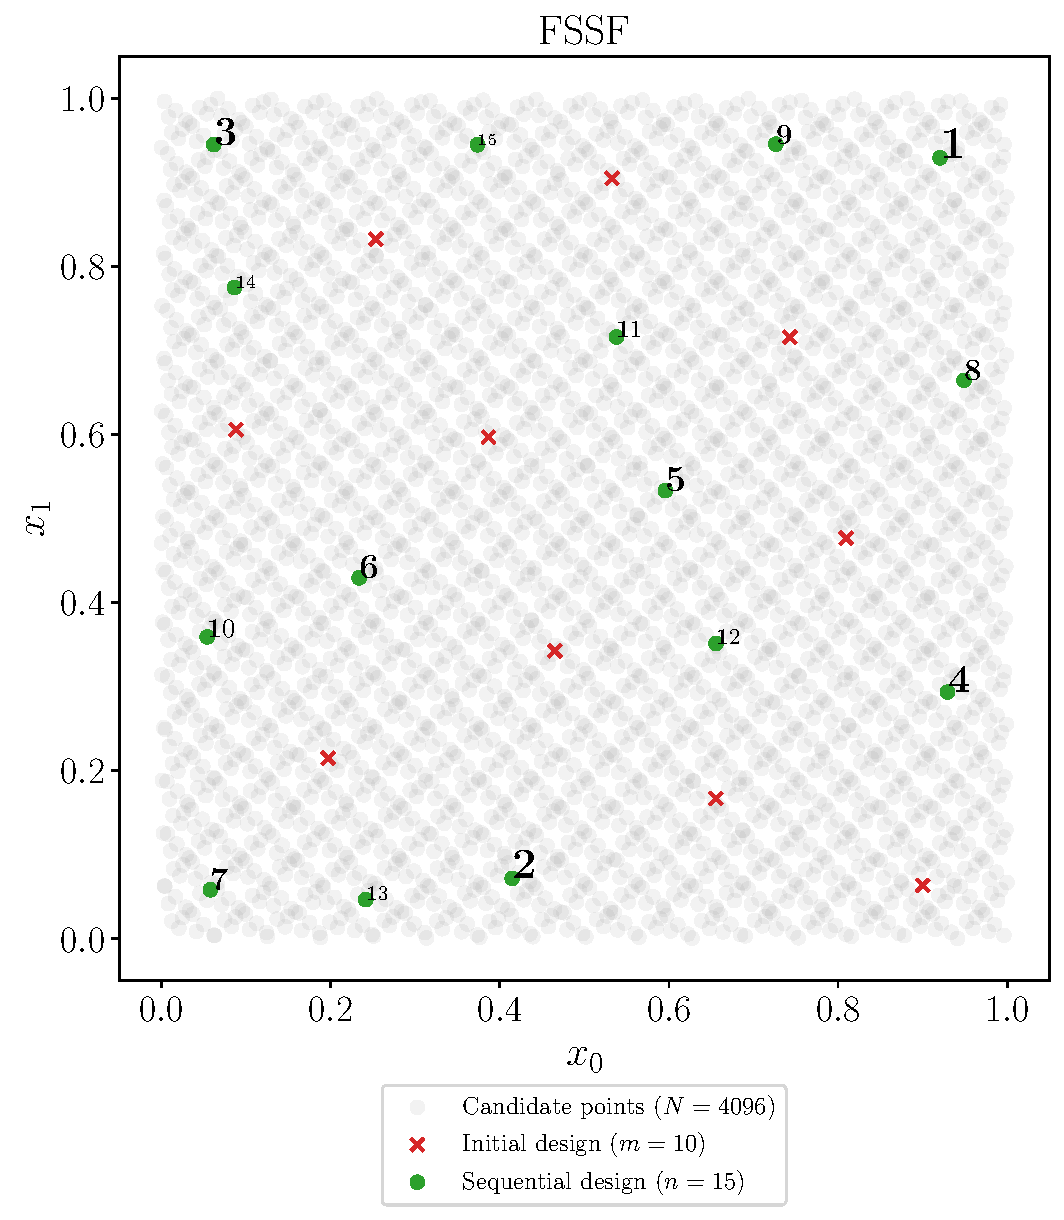
\includegraphics[width=\textwidth]{./part2/figures/SIS/uniform2D_FSSF.pdf}
  \end{subfigure}
  %
  \begin{subfigure}[b]{0.48\linewidth}
    \centering
    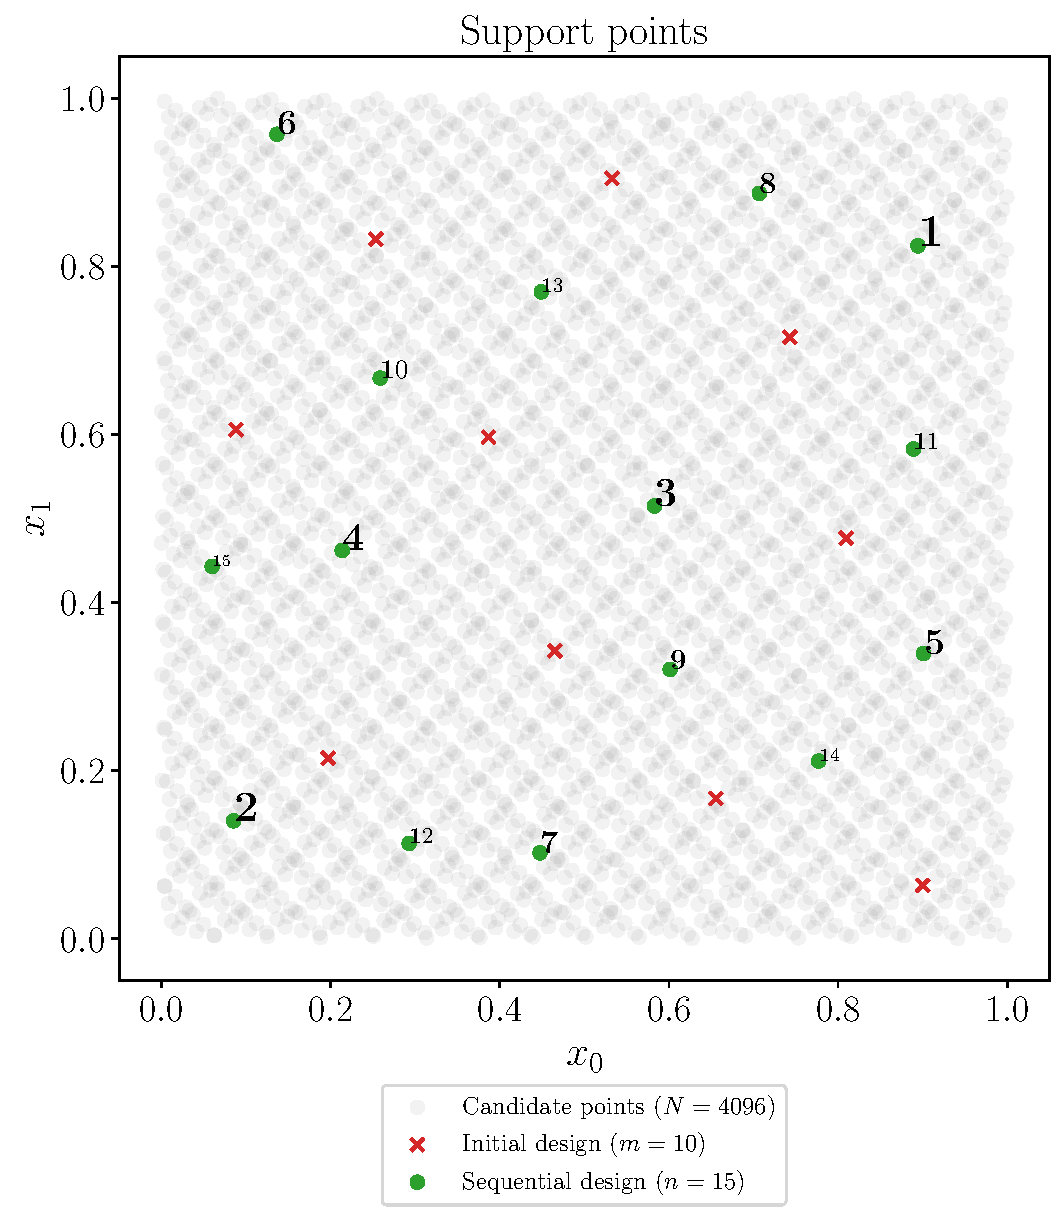
\includegraphics[width=\textwidth]{./part2/figures/SIS/uniform2D_SP.pdf}
  \end{subfigure}
  \\
  \begin{subfigure}[b]{0.48\linewidth}
    \centering
    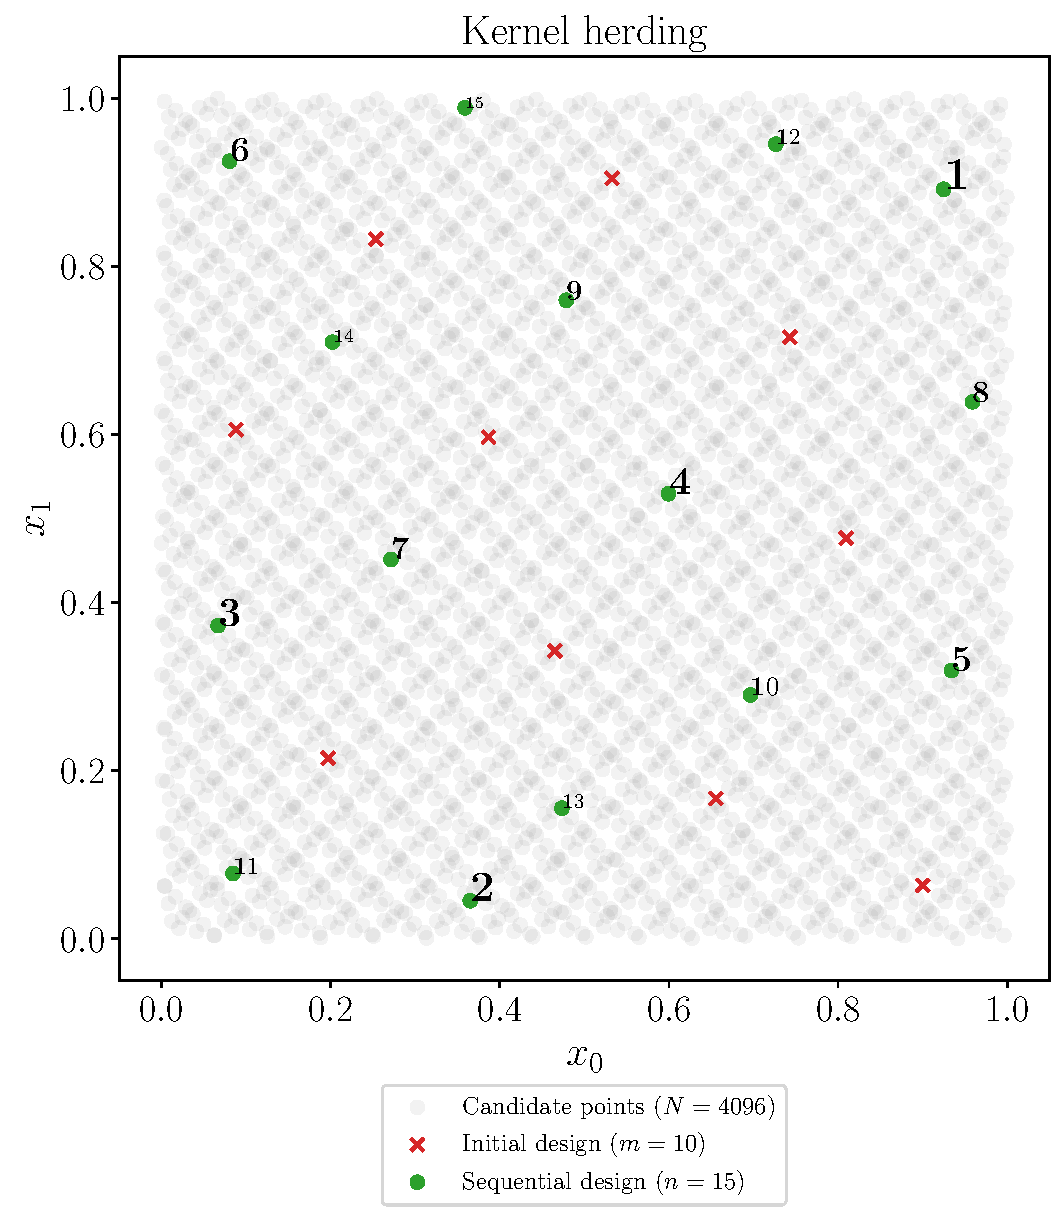
\includegraphics[width=\textwidth]{./part2/figures/SIS/uniform2D_KH.pdf}
  \end{subfigure}
  \caption{Additional points (ordered, green) complementing an initial design (red crosses), $\pi$ is uniform on $[0,1]$, the candidate points are in gray.}
  \label{fig:uniform_validation_designs}
\end{figure}

\begin{figure}
  \centering
  \begin{subfigure}[b]{0.48\linewidth}
    \centering
    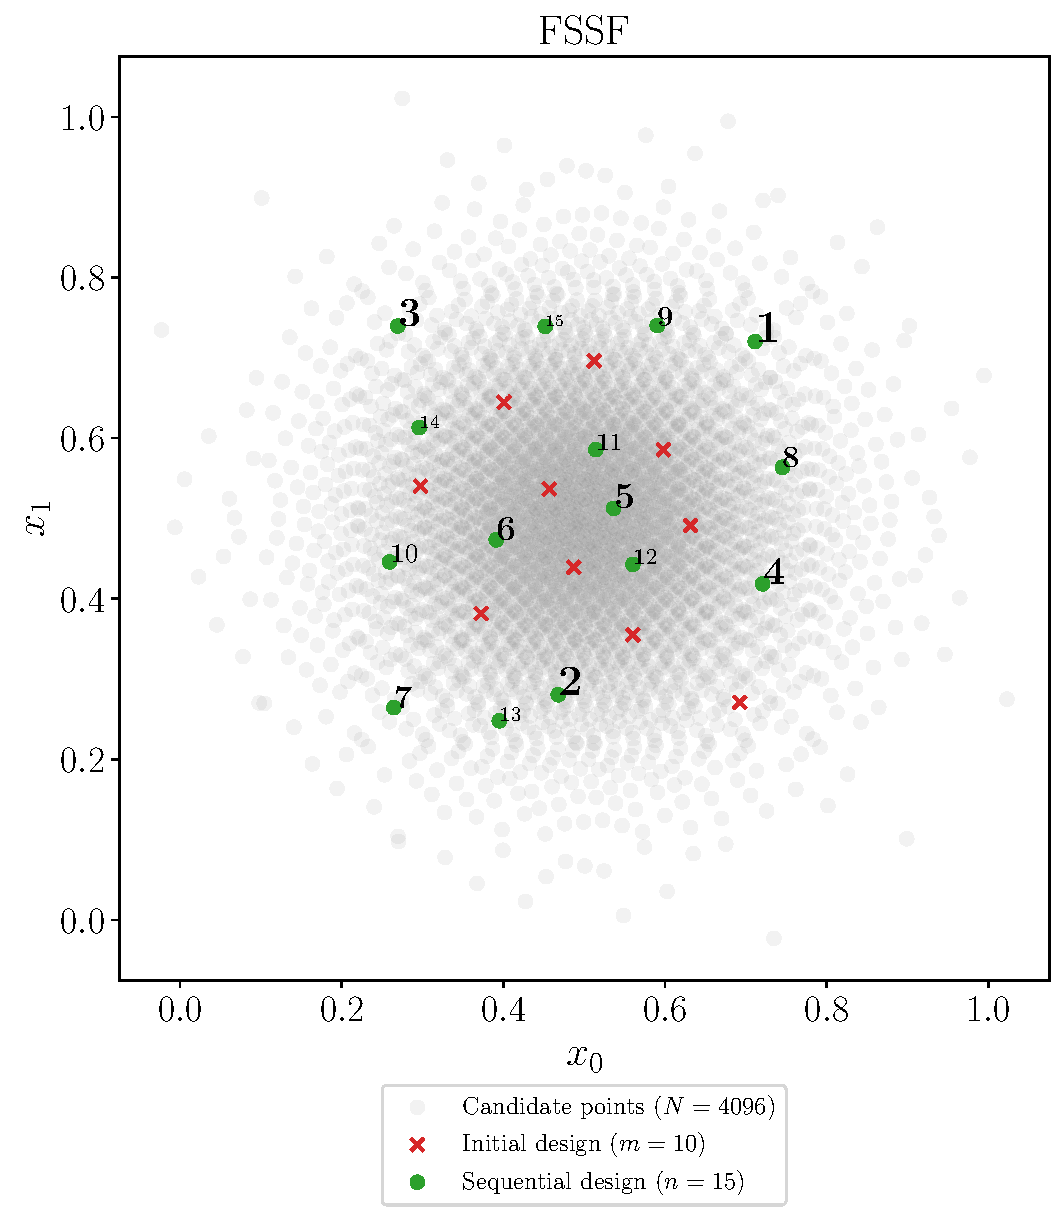
\includegraphics[width=\textwidth]{./part2/figures/SIS/normal2D_FSSF.pdf}
  \end{subfigure}
  %
  \begin{subfigure}[b]{0.48\linewidth}
    \centering
    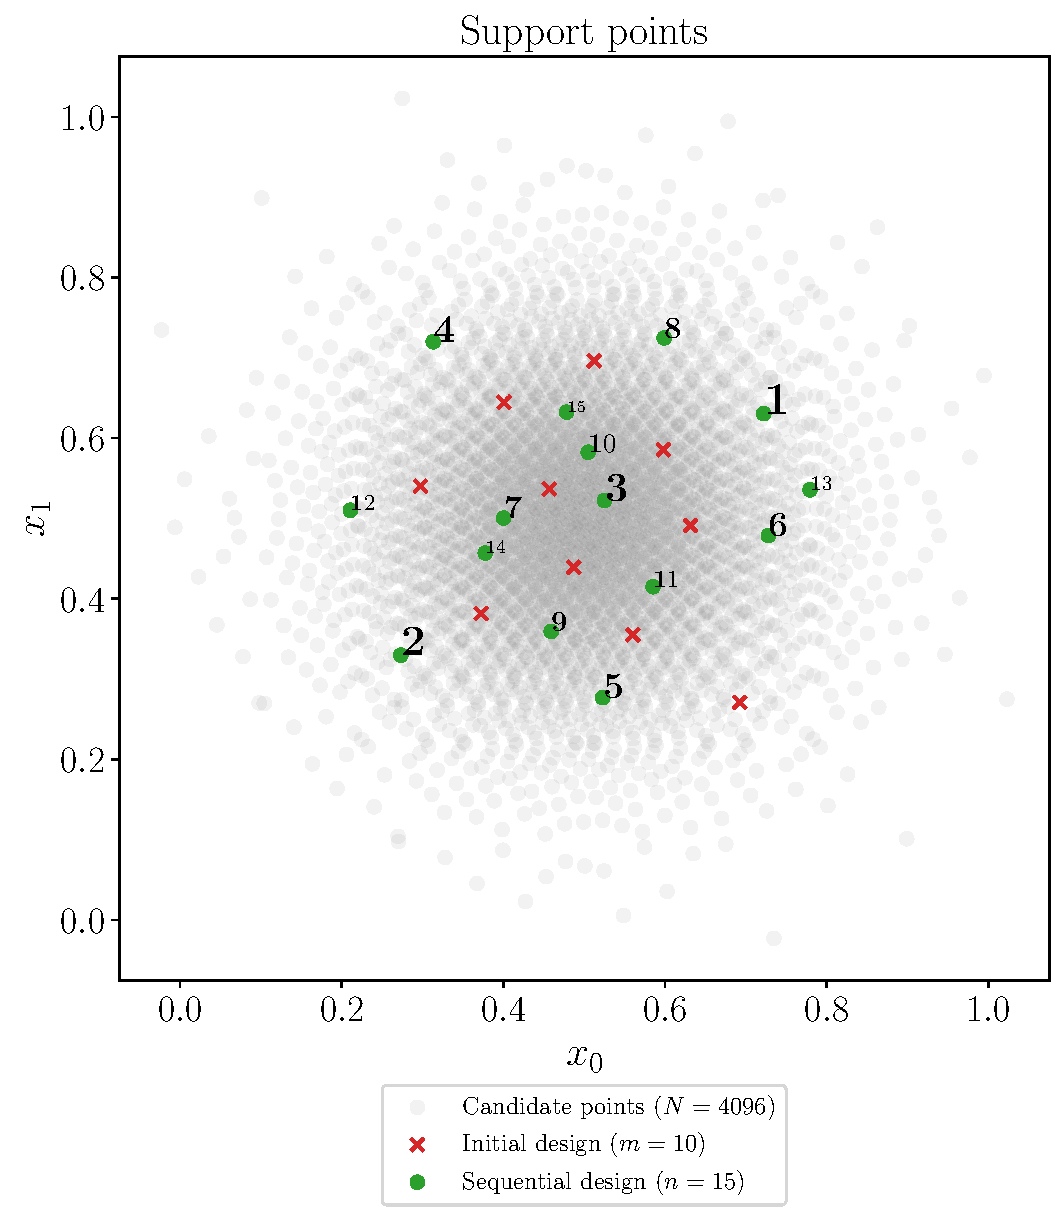
\includegraphics[width=\textwidth]{./part2/figures/SIS/normal2D_SP.pdf}
  \end{subfigure}
  \\
  \begin{subfigure}[b]{0.48\linewidth}
    \centering
    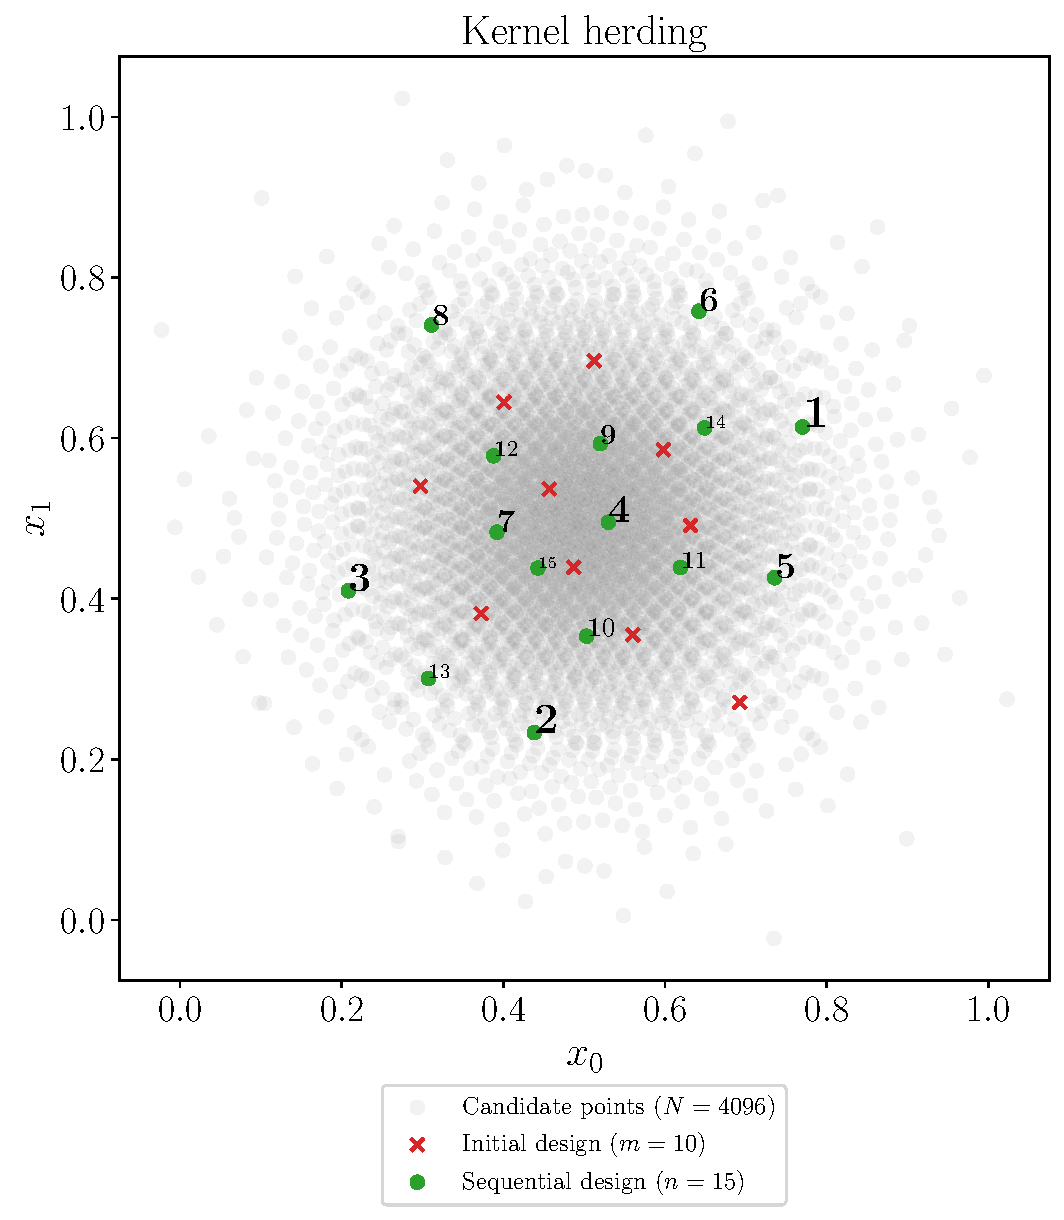
\includegraphics[width=\textwidth]{./part2/figures/SIS/normal2D_KH.pdf}
  \end{subfigure}
  \caption{Additional points (ordered, green) complementing an initial design (red crosses), $\pi$ normal, the candidate points are in gray.}
  \label{fig:normal_validation_designs}
\end{figure}   





%============================================================%
%============================================================%
\section{Numerical experiments I: construction of a training set and a test set}\label{sec:val_res1}
%============================================================%
%============================================================%
This section presents numerical results obtained on three different test cases, in dimension 2 (test cases 1 and 2) and 8 (test case 3), for which $y(\bx)=f(\bx)$ with $f(\bx)$ has an easy to evaluate analytical expression, see Subsection~\ref{sec:testCases}. 
This allows a good estimation of $Q_\pi^2$ (see \eq{eq:Q2th}) by a large Monte Carlo sample (with size $M=10^6$), which will serve as a reference when assessing the performance of each of the other estimators. 

The validation designs are built by FSSF, support points and kernel herding, presented in Subsections~\ref{sec:FSSF},~\ref{sec:SP}, and~\ref{sec:C5_KH}, 
and the performances obtained are compared for each one, considering the uniform and the weighted estimator of Subsection~\ref{sec:weighting}. 

%============================================================%
\subsection{Test cases} \label{sec:testCases}
%============================================================%

The training design $\bX_m$ and the set $\iS$ of potential test set points are as in Subsection~\ref{sec:numerical-1}. 
For test cases 1 and 3, $\pi$ is the uniform measure on $\iD_\bx=[0,1]^d$, with $d=2$ and $d=8$, respectively; $\bX_m$ is a maximin Latin hypercube design in $\iD_\bx$, and $\iS$ corresponds to the first $N$ points $\Sb_N$ of Sobol' sequence in $\iD_\bx$, complemented by the $2^d$ vertices. 
In the second test case, $d=2$, $\pi$ is the normal distribution $\SN(\0b,\Ib_2)$, and the sets $\bX_m$ and $\Sb_N$ must be transformed as explained in Subsection~\ref{sec:FSSF}. 
There are $N=2^{14}$ candidate points for test cases 1 and 2 and $N=2^{15}$ for test case 3 (this value is rather moderate for a problem in dimension 8, but using a larger $N$ yields numerical difficulties for support points; see Subsection~\ref{sec:SP}). 

For each test case, a GP regression model is fitted to the $m$ observations using ordinary Kriging \citep{rasmussen_2006} (a GP model with constant mean), with an anisotropic Matérn kernel with regularity parameter $5/2$, and the correlation lengths $\theta_i$ are estimated by maximum likelihood via a truncated Newton algorithm. 
All calculations were done using the Python package \ot for uncertainty quantification \citep{baudin_dutfoy_2017}. 
The kernel used for kernel herding is different and corresponds to the tensor product of one-dimensional Matérn kernels \eq{eq:Matern5/2}, so that the potentials $P_{\pi}(\cdot)$ are known explicitly (see Appendix~\ref{apx:B}); the correlations lengths are set to $\theta=0.2$ in test cases 1 and 3 ($d=2$) and to $\theta=0.7$ in test case 3 ($d=8$).

Assuming that a model is classified, in terms of the estimated value of its predictivity index $Q^2$ as ``poor fitting'' if $Q^2\in[0.6, 0.8]$, ``reasonably good fitting'', when $Q^2\in(0.8,0.9]$, and ``very good fitting'' if $Q^2>0.9$, for each test case, three different sizes $m$ of the training set are selected such that the corresponding models cover all three possible situations. 
For all test cases, the impact of the size $n$ of the test set is studied in the range $n\in\{4,\ldots,50\}$.

%------------------------------------------------------------%
\paragraph{Test case 1.}
%------------------------------------------------------------%

This test function is $f_1(\bx) = h(2\,x_1 - 1, 2\,x_2 - 1)$, $(x_1,x_2) \in \iD_\bx=[0,1]^2$, with
\begin{align*}
  % t(x_1, x_2) =& (u_1, u_2) ^\intercal = (2x_1 - 1, 2x_2 - 1)^{\intercal} \,.%\\
  h(u_1, u_2) =& \frac{\exp(u_1)}{5} - \frac{u_2}{5} + \frac{u_2^6}{3} + 4 u_2^4 - 4 u_2^2 + \frac{7u_1^2}{10} + u_1^4 + \frac{3}{4 u_1^2 + 4 u_2^2 + 1}\,. %\\
  %g(\bx) =& h \circ t(x_1, x_2)
\end{align*}
Color-coded 3d and contour plots of $f_1$ for $\bX\in\iD_\bx$ are shown on the left panel of \fig{fig:f1&f2}, showing that 
the function is rather smooth, even if its behavior along the boundaries of $\iD_\bx$, in particular close to the vertices, may present difficulties for some regression methods. 
The size of the training set for this function is $m\in\{5, 15, 30\}$.


\begin{figure}
  \centering
  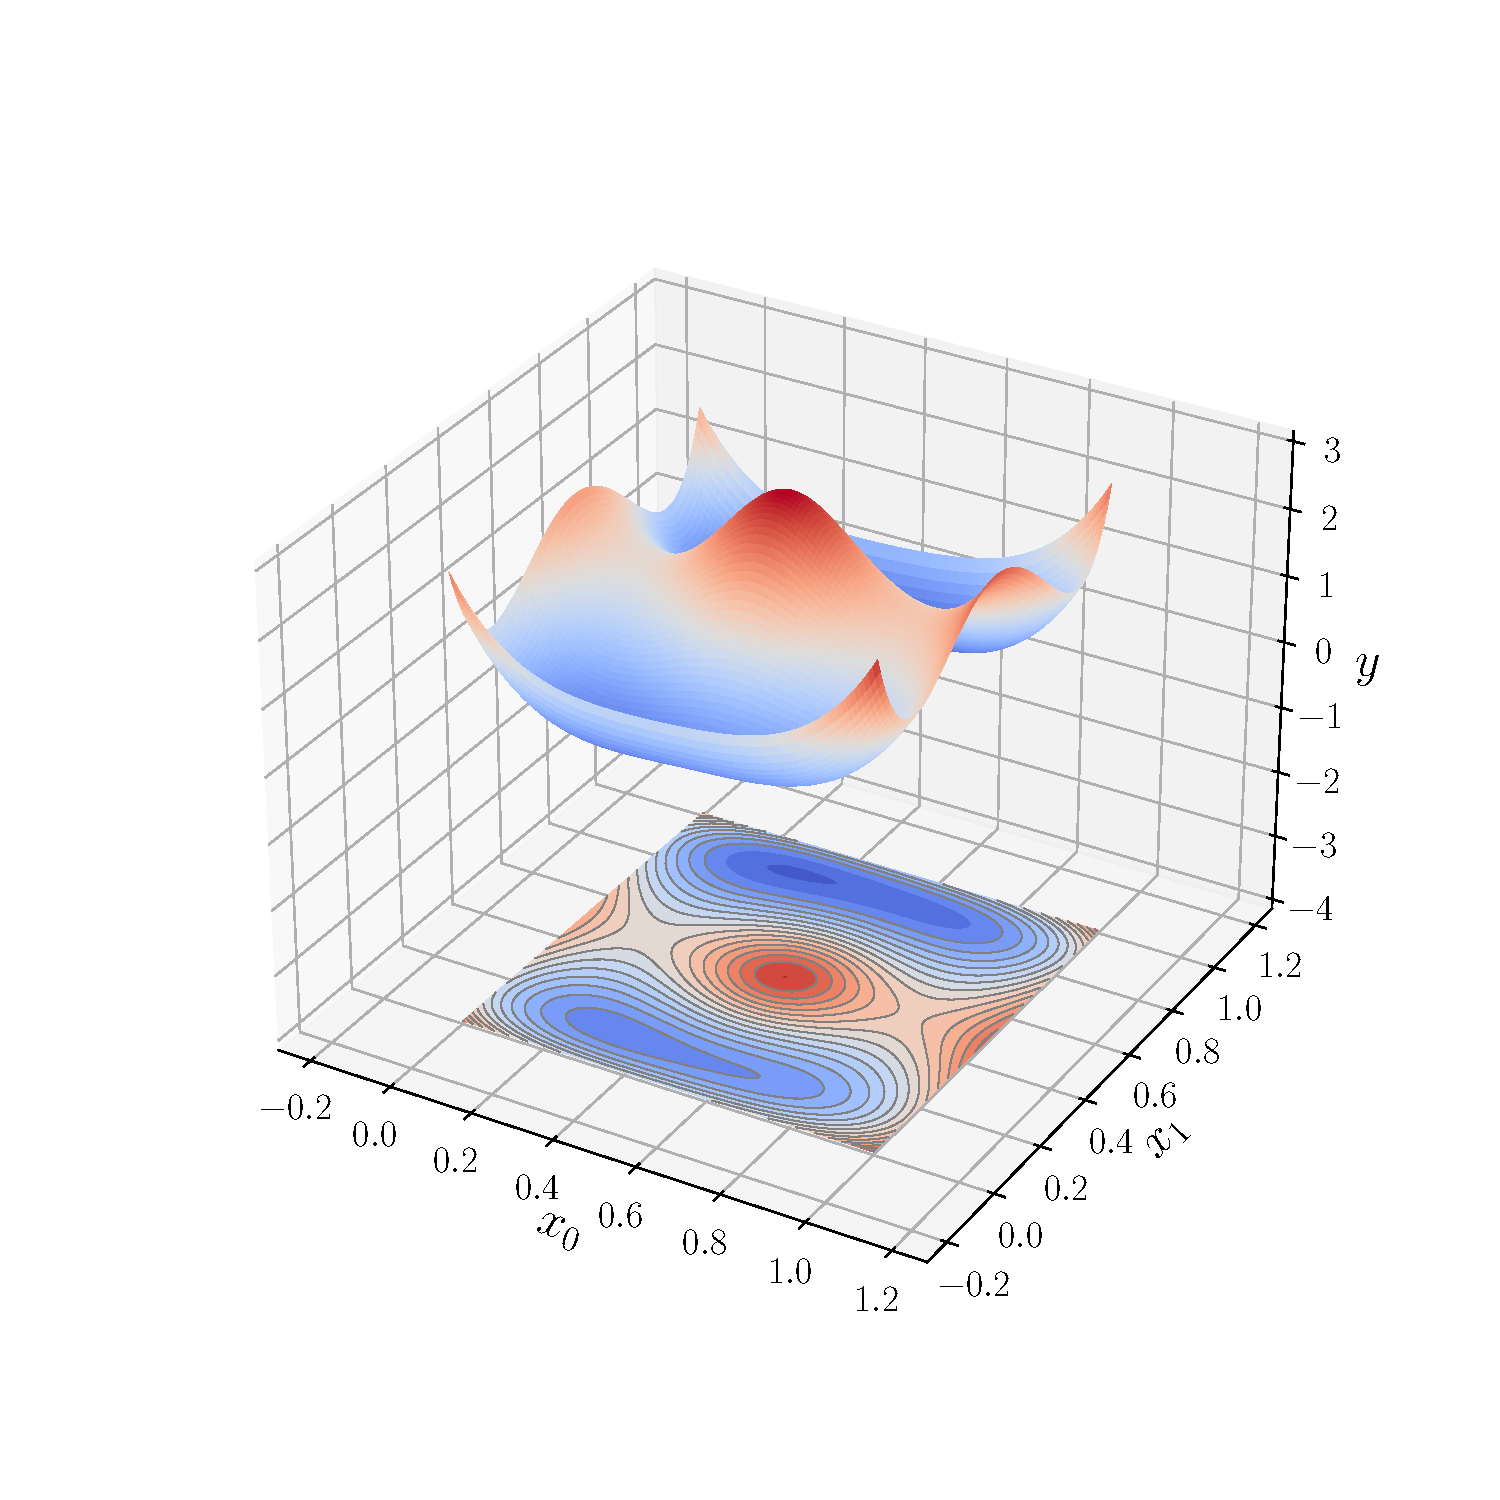
\includegraphics[width=0.49\textwidth]{./part2/figures/SIS/irregular_function3D.pdf}
    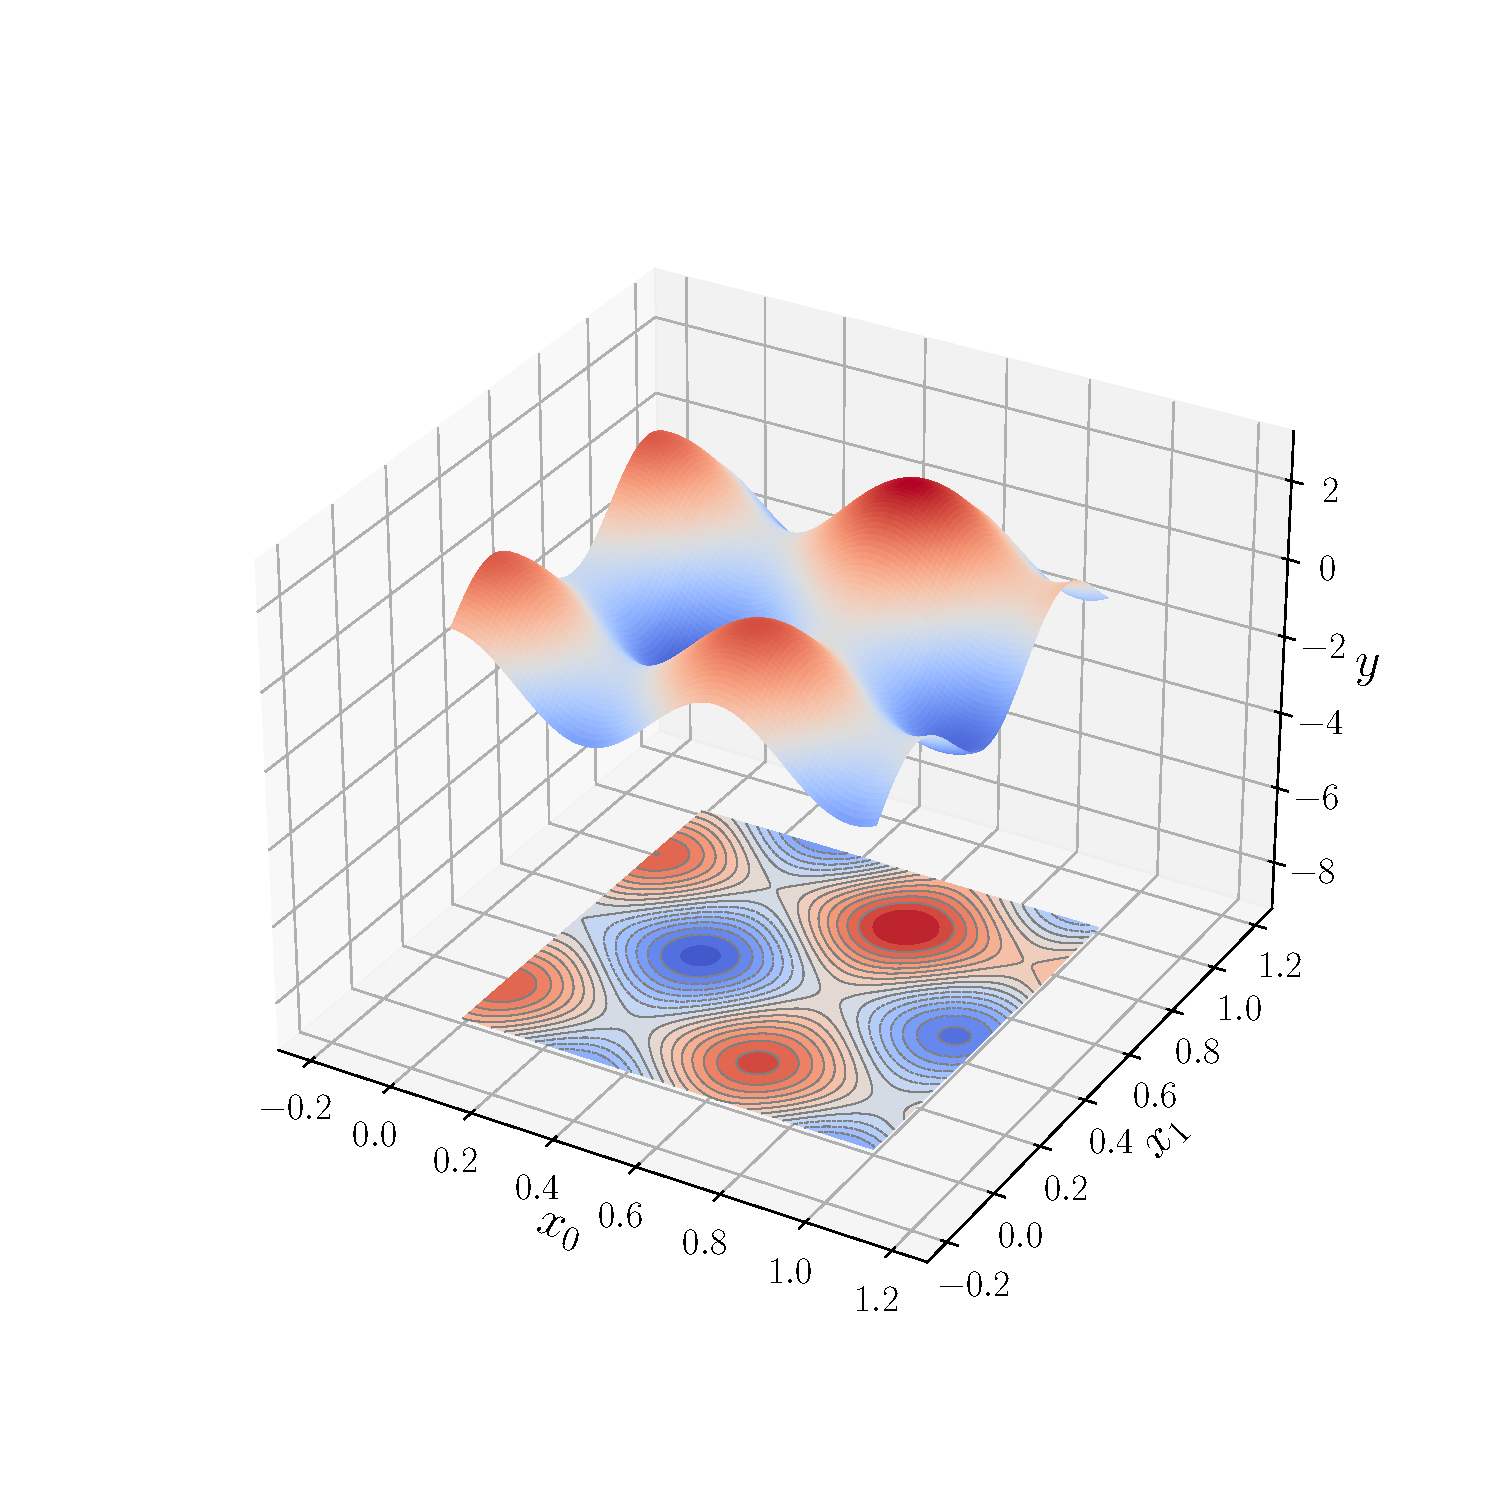
\includegraphics[width=0.49\textwidth]{./part2/figures/SIS/cosin2_function3D.pdf}
  \caption{Left: $f_1(\bx)$ (test case 1); right: $f_2(\bx)$ (test case 2); $\bx\in\iD_\bx=[0,1]^2$.} 
  \label{fig:f1&f2}
\end{figure}


%------------------------------------------------------------%
\paragraph{test case 2.}
%------------------------------------------------------------%

The second test function, plotted in the right panel of \fig{fig:f1&f2} for $\bx\in[0,1]^2$, is 
\begin{align*}
   f_2(\bx) 
   %&= \cos(10(0.5 + 0.15 x_1)) + \sin(10 (0.5 + 0.15 x_2)) + (0.5 + 0.15 x_1) (0.5 + 0.15 x_2) \\
   &= \cos \left(5 + \frac{3}{2}x_1 \right) + \sin \left(5 + \frac{3}{2}x_1 \right) 
   + \frac{1}{100} \left(5 + \frac{3}{2}x_1 \right) \left(5 + \frac{3}{2}x_2 \right)\,.
\end{align*}
%The measure $\pi$ is the standard bivariate normal distribution $\SN(\0b,\Ib_2)$ on $\iD_\bx=\R^2$. 
Training set sizes for this test case are $m\in\{8, 15, 30\}$.

%------------------------------------------------------------%
\paragraph{test case 3.}
%------------------------------------------------------------%

The third function is the so-called ``gSobol'' function, defined over $\iD_\bx=[0,1]^8$ by
\begin{equation*}
  f_3(\bx) = \prod_{i=1}^{8} \frac{|4x_i - 2| + a_i}{1 + a_i}, \qquad a_i = i^2 \,.
\end{equation*}
%and $\pi$ is the uniform measure on the 8-dimensional unit hyper-cube. 
This parametric function is very versatile as both the dimension of its input space and the coefficients $a_i$ can be freely chosen. 
The sensitivity to input variables is determined by the $a_i$: the larger $a_i$ is, the less $f$ is sensitive to $x_i$. 
Larger training sets are considered for this test case: $m\in\{15, 30, 100\}$.

%============================================================%
\subsection{Benchmark results and analysis}
%============================================================%

The numerical results obtained in this section are presented in Figures~\ref{fig:irregular_benchmark}, \ref{fig:cosin_benchmark}, and \ref{fig:gsobol_benchmark}. 
Each figure corresponds to one of the test cases and gathers three sub-figures, corresponding to test sets with sizes $m$ yielding poor (left), reasonably good (right) or very good (bottom) fittings. 
 
The baseline value of $Q_{MC}^2$, calculated with $10^6$ Monte Carlo points, is indicated by the black diamonds (the black horizontal lines).
Assuming that the error of $Q_{MC}^2$ is much smaller than the errors of all other estimators, this section compares the ability of the methods to approximate $Q_{MC}^2$. 
For each sequence of nested test sets ($n\in\{4,\ldots,50\}$), the observed values of $\widehat Q^2_n$ (equation \eq{eq:Q2test}) and $Q_{n*}^2$ (equation \eq{Q2-est*}), are plotted as the solid and dashed lines, respectively. 

The figures also show the value $Q^2_{\mathrm{LOO}}$ obtained by Leave-One-Out (LOO) cross-validation, which is indicated at the left of each figure by a red diamond (values smaller than $0.25$ are not shown). 
Note that, contrarily to the other methods considered, for LOO the test set is not disjoint from the training set, and thus the method does not satisfy the conditions set in the Introduction. 
As the complete model-fitting procedure is repeated for each training sample of size $m-1$, including the maximum-likelihood estimation of the correlation lengths of the Matérn kernel, the closed-form expressions of \citet{Dubrule83} cannot be used, making the computations rather intensive. 
The three figures show, and as expected, that the $Q_{LOO}^2$ tends to under-estimate $Q_{\mathrm{ideal}}^2$: by construction of the training set, LOO cross-validation relies on model predictions at points $\bx^{(i)}$ far from the other $m-1$ design points used to build the model, and thus tends to systematically overestimate the prediction error at $\bx^{(i)}$. 
The underestimation of $Q_{\mathrm{ideal}}^2$ can be particularly severe when $m$ is small, the training set is then necessarily sparse; see \fig{fig:irregular_benchmark} where $Q_{LOO}^2<0.3$ for $m=5$ and 15. 

Let us first concentrate on the non-weighted estimators (solid curves). 
The two MMD-based constructions, support points (in orange) and kernel herding (in blue), generally produce better validation designs than FSSF (green curves), leading to values of $\widehat Q^2_n$ that approach $Q_{\mathrm{ideal}}^2$ quicker as $n$ increases. 
This is particularly noticeable for ``good'' and ``very good'' models (central and rightmost panels of all three figures). 
This supports the idea that test sets should complement the training set $\bX_m$ by populating the holes it leaves in $\iD_\bx$ while at the same time being able to mimic the target distribution $\pi$, this second objective being more difficult to achieve for FSSF than for the MMD-based constructions. 

A comparison of the two MMD-based estimators reveals that support points tend to underestimate ISE, leading to an over-confident assessment of the model predictivity, while kernel herding displays the expected behavior, with a negative bias that decreases with $n$. 
The reason for the positive bias of estimates based on support points designs is not fully understood, but may be linked to the fact that support points tend to place validation points at ``mid-range'' from the designs (and not at the furthest points like FSSF or kernel herding), see central and rightmost panels in Figure \ref{fig:uniform_validation_designs}, and thus residuals at these points are themselves already better representatives of the local average errors. 

Let us consider now the impact of the GP-based weighting of the residuals when estimating $Q^2$ (by $Q_{n*}^2$), which is related to the relative training-set/validation-set geometry (the manner in which the two designs are entangled in ambient space). 
The improvement resulting from applying residual weighting is apparent on all panels of the three figures, the dashed curves lying closer to $Q_{\mathrm{ideal}}^2$ than their solid counterparts; see in particular kernel herding (blue curve) in \fig{fig:irregular_benchmark} and FSSF (green curve) in \fig{fig:cosin_benchmark}. 
Unexpectedly, the estimators based on support points seem to be rather insensitive to residual weighting, the dashed and solid orange curves being most of the time close to each other (and in any case, much closer than the green and blue ones). 
While the reason for this behavior deserves a deeper study, the fact that the support point designs -- see Figure \ref{fig:uniform_validation_designs} -- sample in a better manner the range of possible training-to-validation distances, being in some sense less space-filling than both FSSF and kernel herding, is again a plausible explanation for this weaker sensitivity to residual weighting.


Consider now a comparison of the behavior across test cases. 
Setting aside the strikingly singular situation of test case 2, for which kernel herding displays a pathological (bad) behavior for the ``very good'' model, 
and all methods present an overall good behavior, 
the details of the tested function do not seem to play an important role concerning the relative merits of the estimators and validation designs.

\begin{figure}
  \centering
  \begin{subfigure}[b]{0.49\linewidth}
    \centering
    % Poor metamodel
    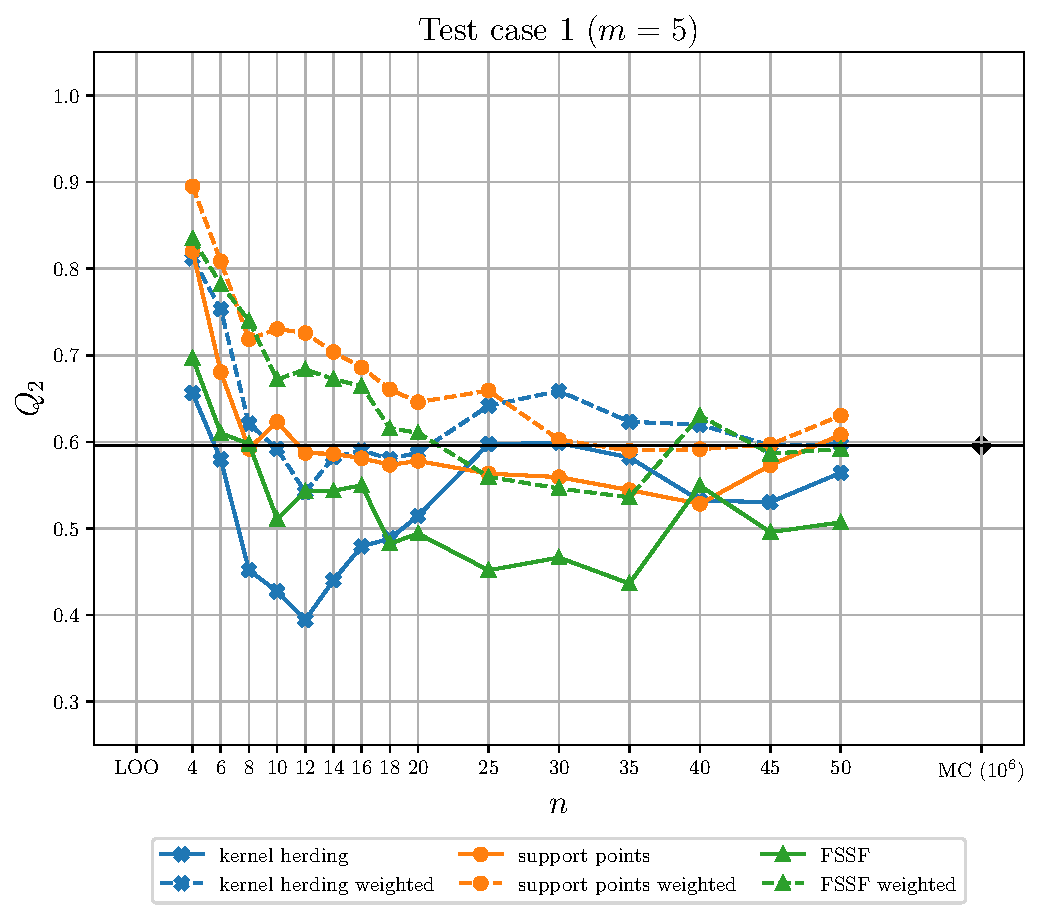
\includegraphics[width=\linewidth]{./part2/figures/SIS/irregular_learnsize_5.pdf}
  \end{subfigure}
  %
  \centering
  \begin{subfigure}[b]{0.49\linewidth}
    \centering
    % Good metamodel
    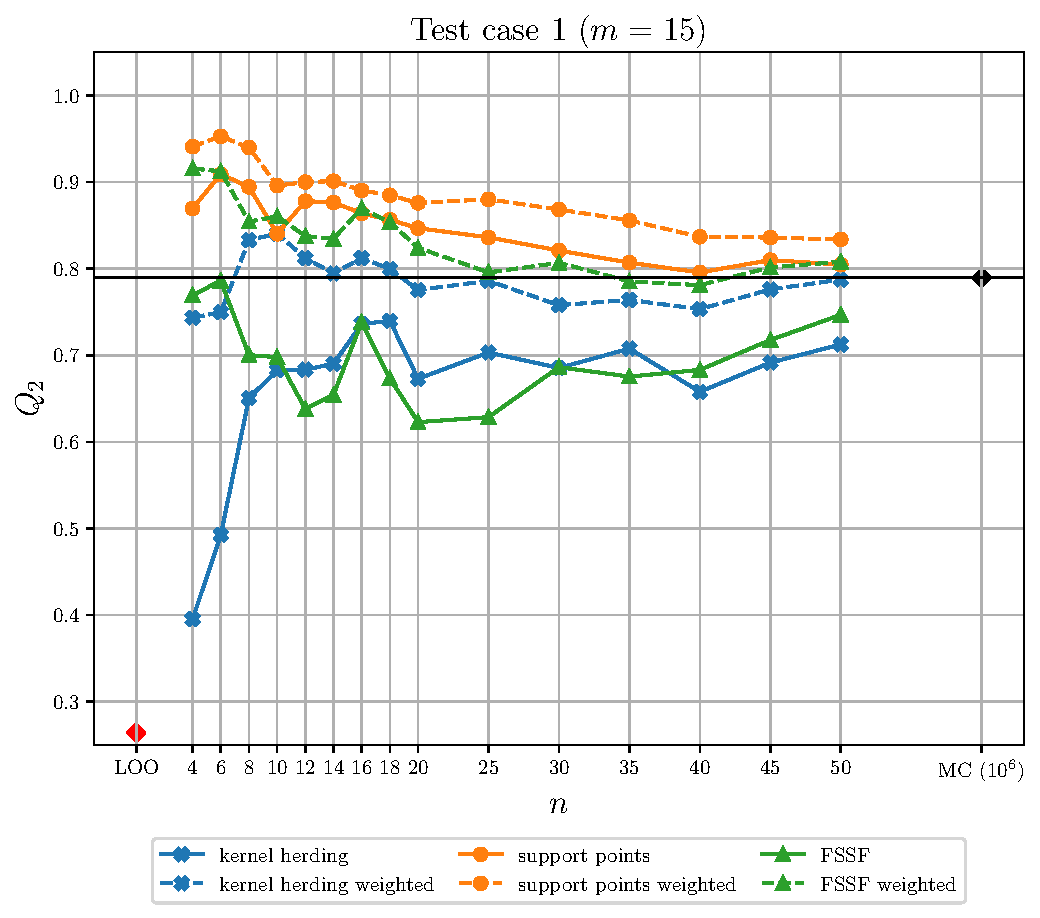
\includegraphics[width=\linewidth]{./part2/figures/SIS/irregular_learnsize_15.pdf}
  \end{subfigure}
  \\
  \centering
  \begin{subfigure}[b]{0.49\linewidth}
    \centering
    % Perfect metamodel
    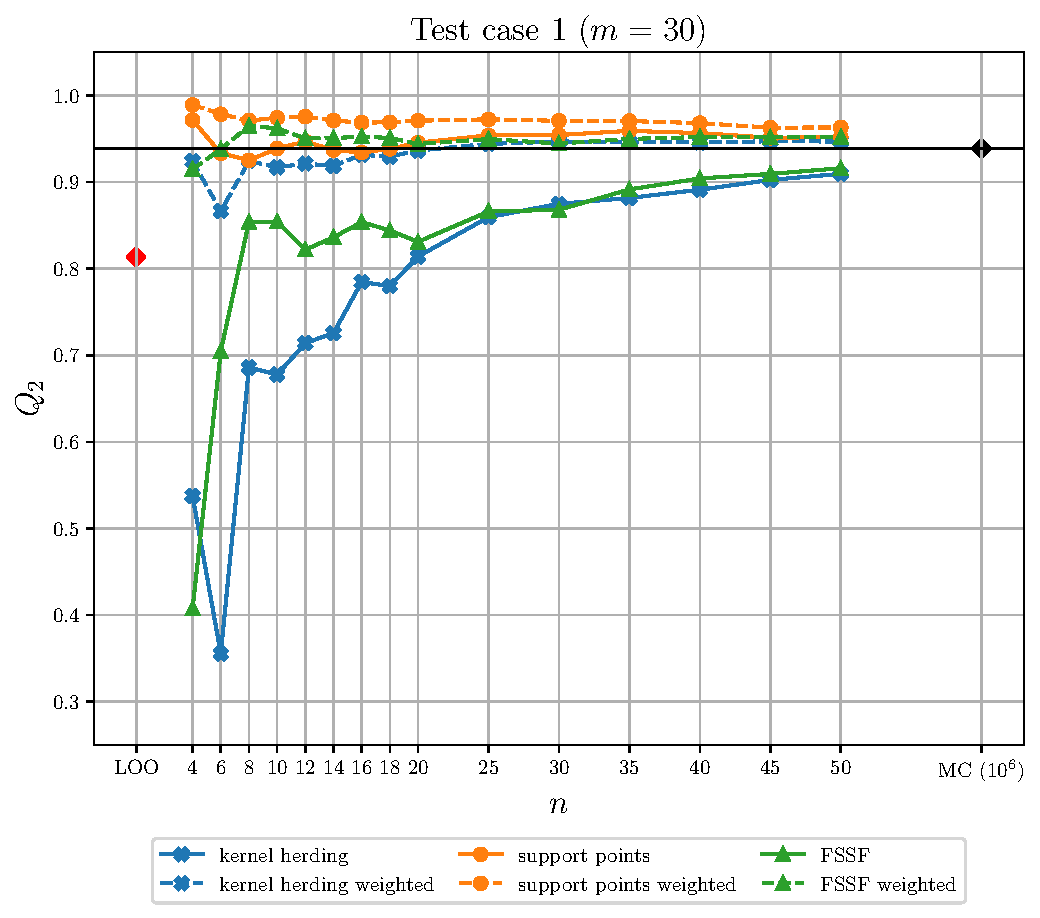
\includegraphics[width=\linewidth]{./part2/figures/SIS/irregular_learnsize_30.pdf}
  \end{subfigure}
  \caption{test case 1: predictivity assessment of a poor (left), good (right) and very good (bottom) model with kernel herding, support points and FSSF test sets.}
  \label{fig:irregular_benchmark}
\end{figure}



\begin{figure}
  \centering
  \begin{subfigure}[b]{0.49\linewidth}
    \centering
    % Poor metamodel
    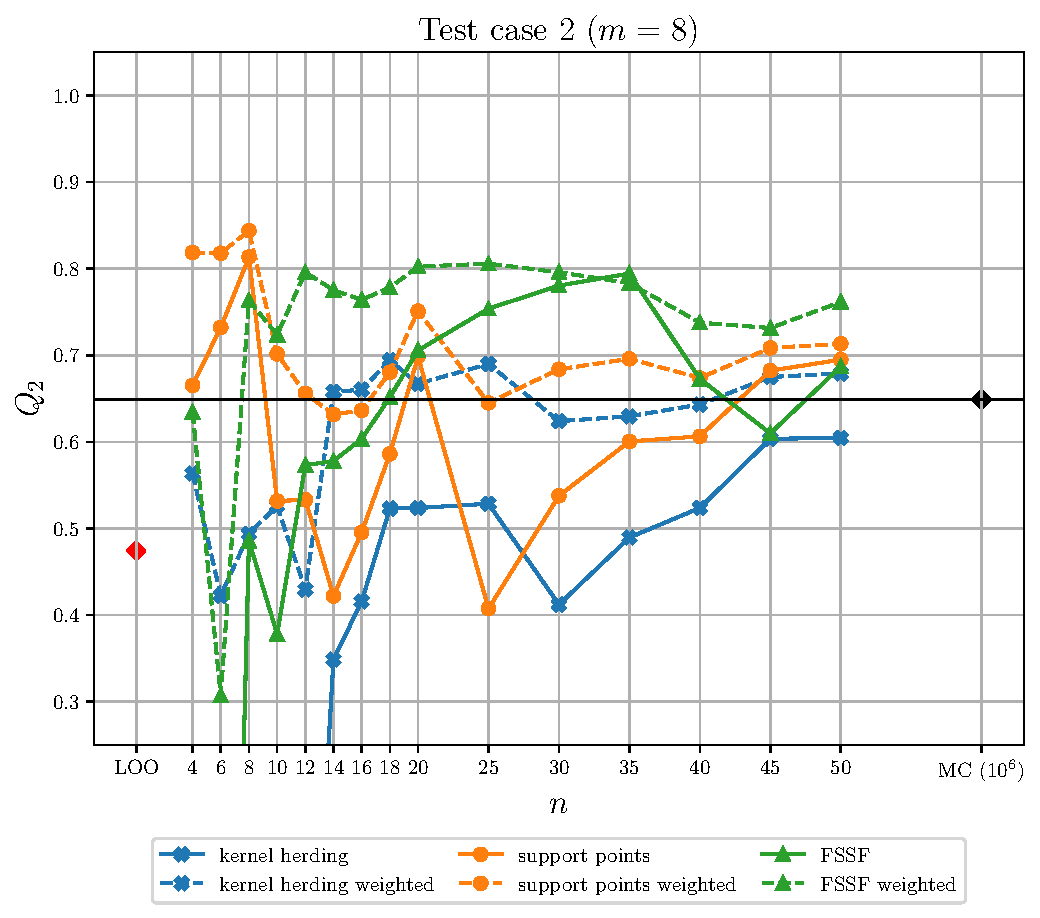
\includegraphics[width=\linewidth]{./part2/figures/SIS/cosin_learnsize_8.pdf}
  \end{subfigure}
  %
  \centering
  \begin{subfigure}[b]{0.49\linewidth}
    \centering
    % Good metamodel
    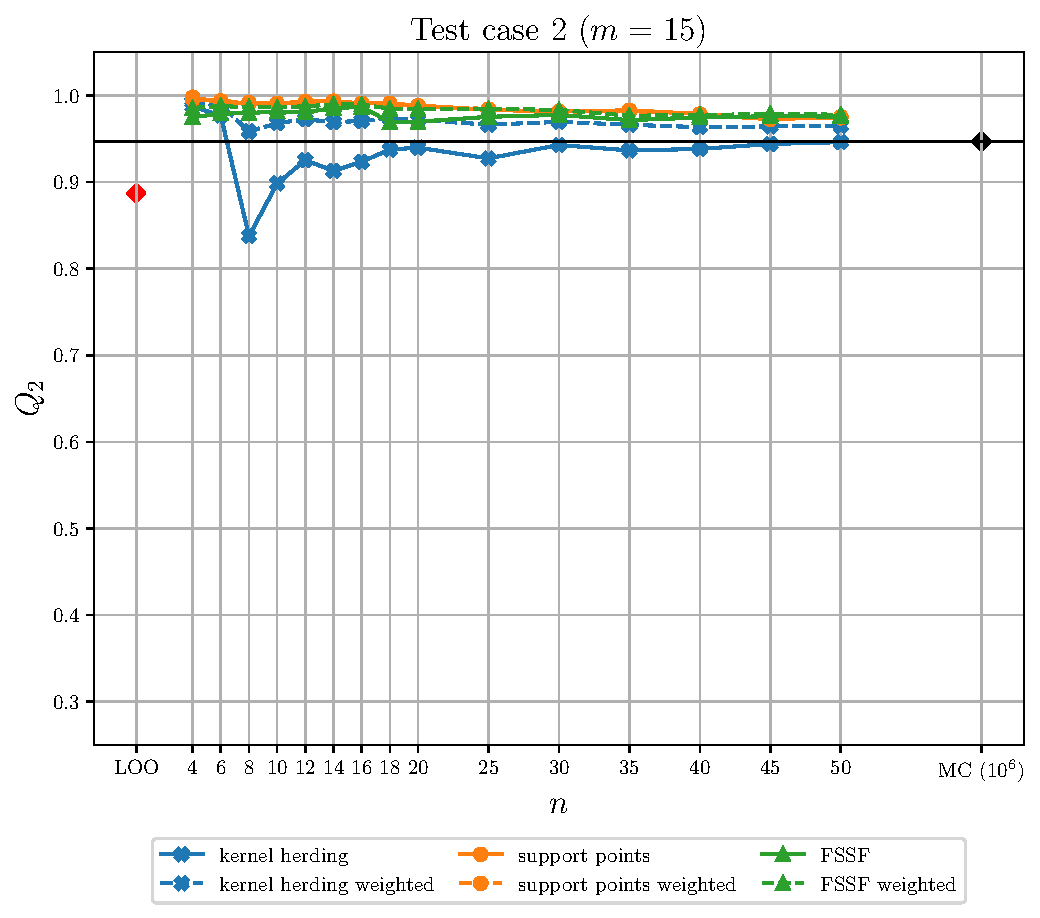
\includegraphics[width=\linewidth]{./part2/figures/SIS/cosin_learnsize_15.pdf}
  \end{subfigure}
  %
  \centering
  \begin{subfigure}[b]{0.49\linewidth}
    \centering
    % Perfect metamodel
    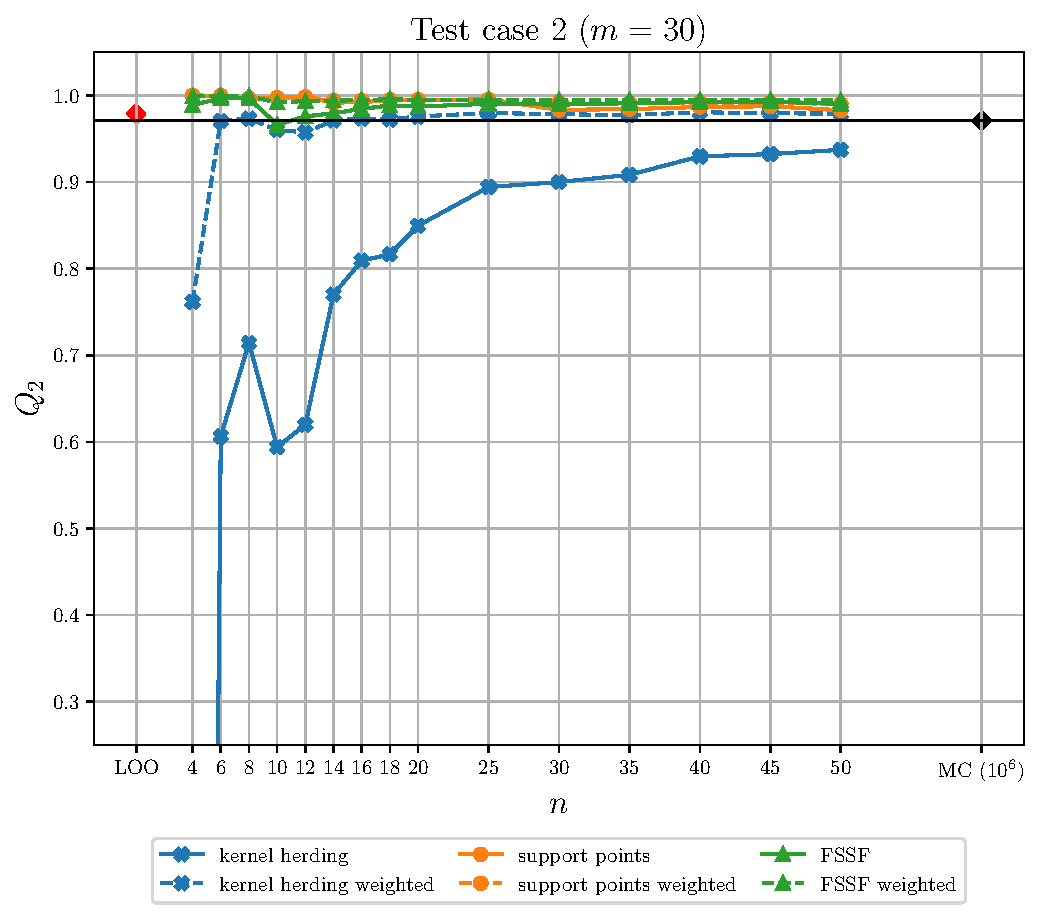
\includegraphics[width=\linewidth]{./part2/figures/SIS/cosin_learnsize_30.pdf}
  \end{subfigure}
  \caption{test case 2: predictivity assessment of a poor (left), good (right) and very good (bottom) model with kernel herding, support points and FSSF test sets.}
  \label{fig:cosin_benchmark}
\end{figure}

\begin{figure}
  \centering
  \begin{subfigure}[b]{0.49\linewidth}
    \centering
    % Poor metamodel
    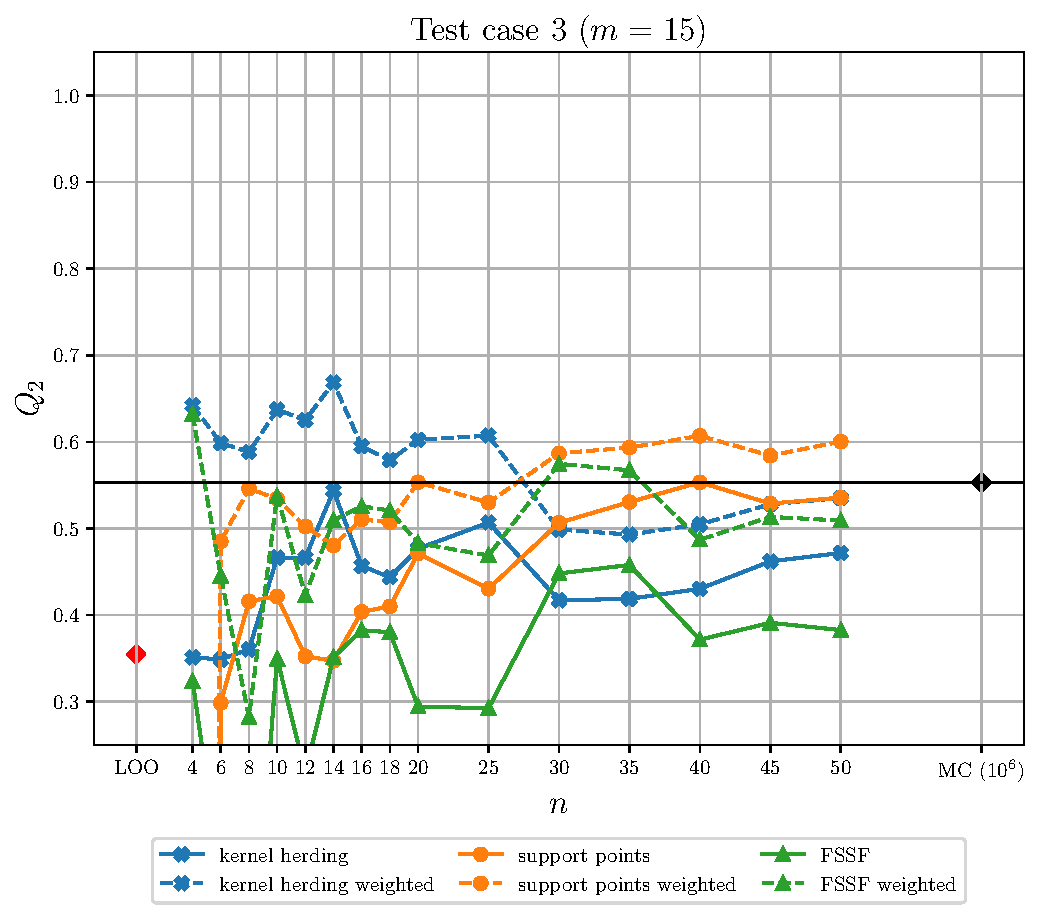
\includegraphics[width=\linewidth]{./part2/figures/SIS/gsobol_learnsize_15.pdf}
  \end{subfigure}
  %
  \centering
  \begin{subfigure}[b]{0.49\linewidth}
    \centering
    % Good metamodel
    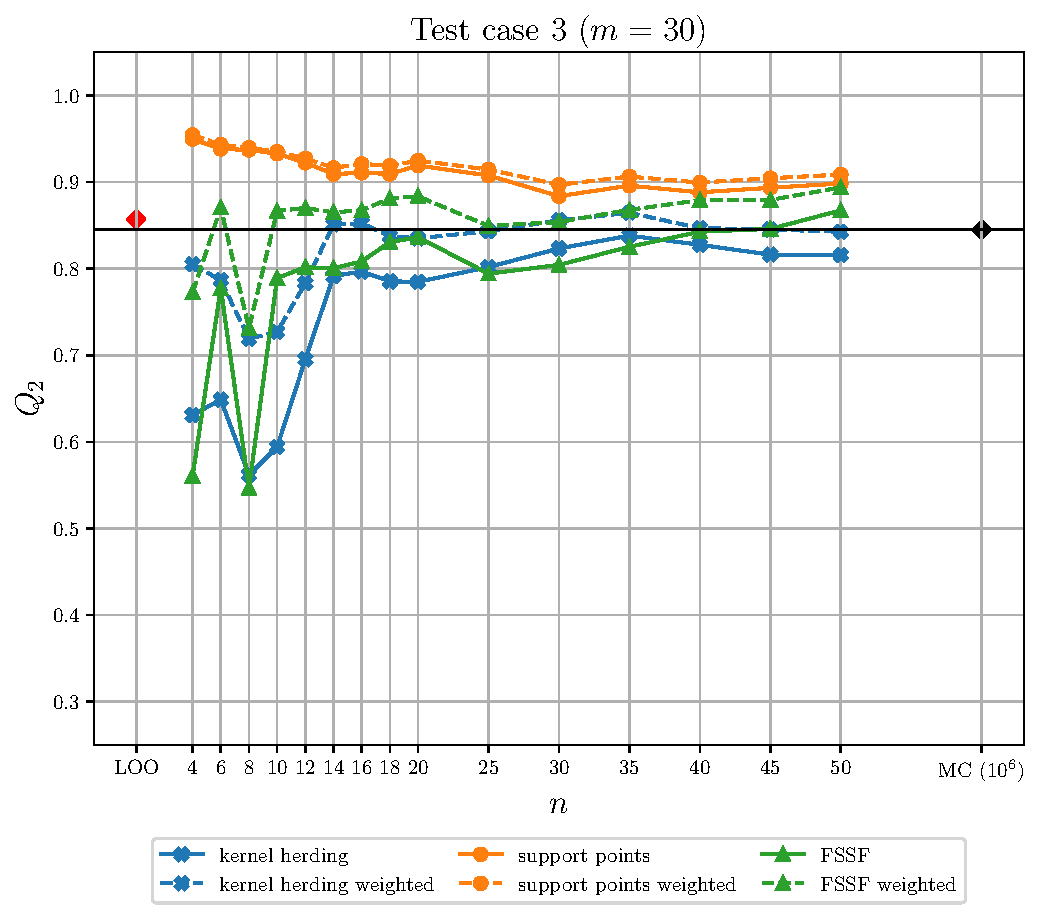
\includegraphics[width=\linewidth]{./part2/figures/SIS/gsobol_learnsize_30.pdf}
  \end{subfigure}
  \\
  \centering
  \begin{subfigure}[b]{0.49\linewidth}
    \centering
    % Perfect metamodel
    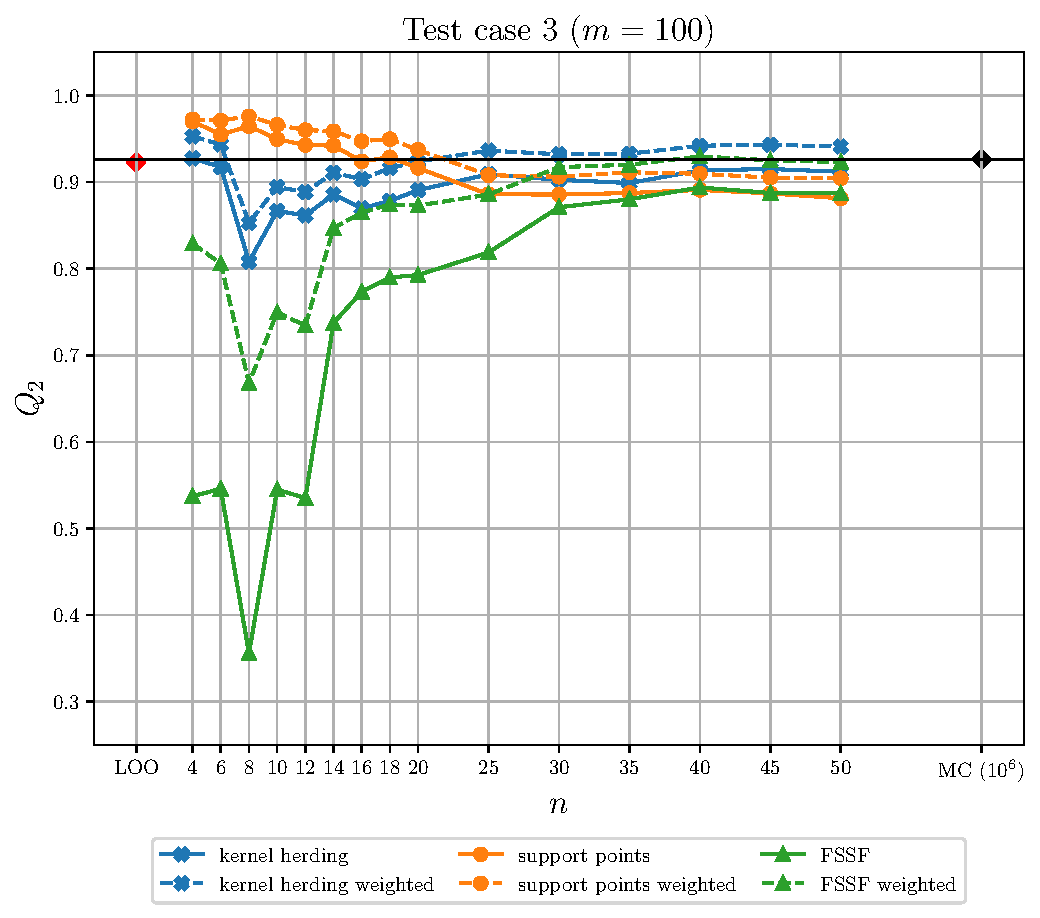
\includegraphics[width=\linewidth]{./part2/figures/SIS/gsobol_learnsize_100.pdf}
  \end{subfigure}
  \caption{test case 3: predictivity assessment of a poor (left), good (right) and very good (bottom) model with kernel herding, support points and FSSF test sets.}
  \label{fig:gsobol_benchmark}
\end{figure}

Let us finally observe how the methods behave for models of distinct quality ($m$ leading to poor, good or very good models), comparing the three panels in each figure. 
On the left panels, $m$ is too small for the model $\eta_m$ to be accurate, and all methods and test-set sizes are able to detect this. 
For models of practical interest (good and very good), the test sets generated with support points and kernel herding allow a reasonably accurate estimation of $Q^2$ with a few points. 
Note, incidentally, that except for test case 2 (where the interplay with a non-uniform measure $\pi$ complicates the analysis), it is in general easier to estimate the quality of the very good model (right-most panel) than that of the good model (central panel), indicating that the expected complexity (the entropy) of the residual process should be a key factor determining how large the validation set must be. 
In particular, it may be that larger values of $m$ allow for smaller values of $n$.





%============================================================%
%============================================================%
\section{Numerical experiments II: splitting a dataset into a training set and a test set}\label{sec:val_res2}
%============================================================%
%============================================================%
This section illustrates the performance of the different designs and estimators considered in this chapter when applied in the context of an industrial application, to split a given dataset of size $N$ into training and test sets, with $m$ and $n$ points respectively, $m+n=N$. 
In contrast with \citet{josvak21}, the observations $y(\bx^{(i)})$, $i=1,\ldots,N$, are not used in the splitting mechanism, meaning that it can be performed before the observations are collected and that there cannot be any selection bias related to observations 
(indeed, the use of observation values in an MMD-based splitting criterion may favor the allocation of the most different observations to different sets, training versus validation).

An ML model is fitted to the training data, and the data collected on the test set are used to assess the predictivity of the model. 
The influence of the ratio $r_n=n/N=1-m/N$ on the quality assessment is investigated. 
Random Cross-Validation (\abv{rcv}) is also considered, where $n$ points are chosen at random among the $N$ points of the dataset: for each $n$, there are $N \choose n$ possible choices, and $R=1\,000$ designs were randomly selected among them. 
A model is fitted on the $m$ complementary points ($m=N-n$), which yields an empirical distribution of $Q^2$ values for each ratio $n/N$ considered. 

%============================================================%
\subsection{Industrial test case CATHARE}
%============================================================%

The test case corresponds to the computer code CATHARE2 (for ``Code Avanc\'e de ThermoHydraulique pour les Accidents de R\'eacteurs \`a Eau''), which models the thermal-hydraulic behavior inside nuclear pressurized water reactors \citep{gefant11}. 
The studied scenario simulates a hypothetical large-break loss of primary coolant accident for which the output of interest is the peak cladding temperature \citep{decbaz08,ioobou10}. 
The complexity of this application lies in the large run-time of the computer model (of the order of twenty minutes) and in the high dimension of the input space: the model involves $53$ input parameters $z_i$, corresponding mostly to constants of physical laws, but also coding initial conditions, material properties and geometrical modeling. 
The $z_i$ were independently sampled according to normal or log-normal distributions. %(see axes histograms in \fig{fig:cathare_paiplot} corresponding to $10$ inputs). 
These characteristics make this test case challenging in terms of construction of a surrogate model and validation of its predictivity.


%\begin{figure}
%  \centering
%  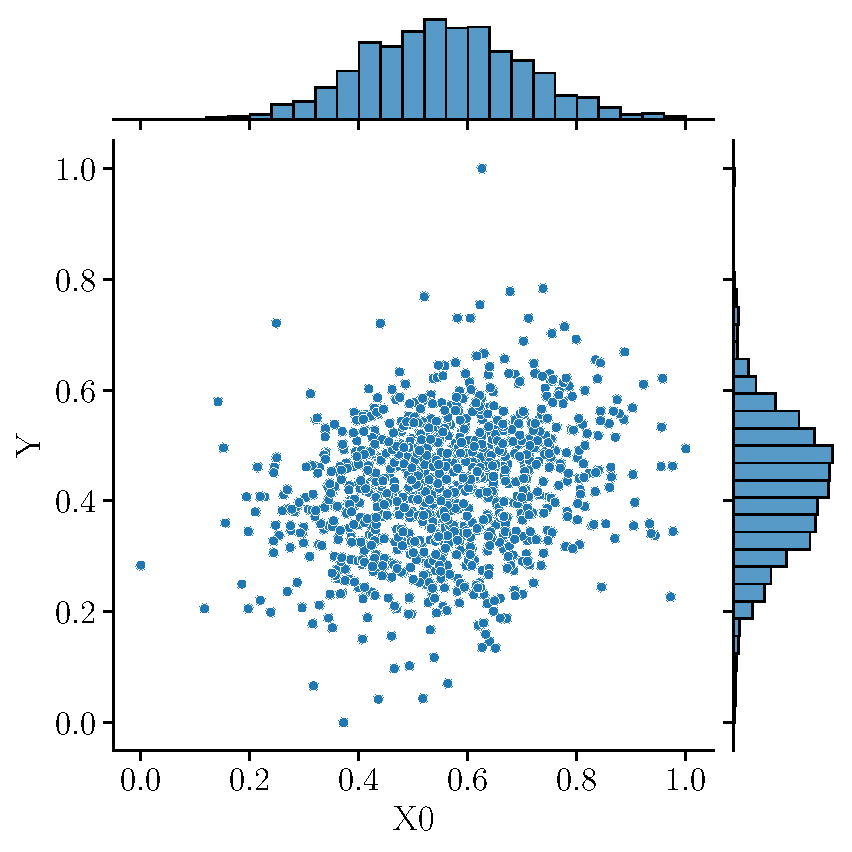
\includegraphics[width=0.32\textwidth]{./part2/figures/SIS/cathare_jointplot_X0.pdf}
%  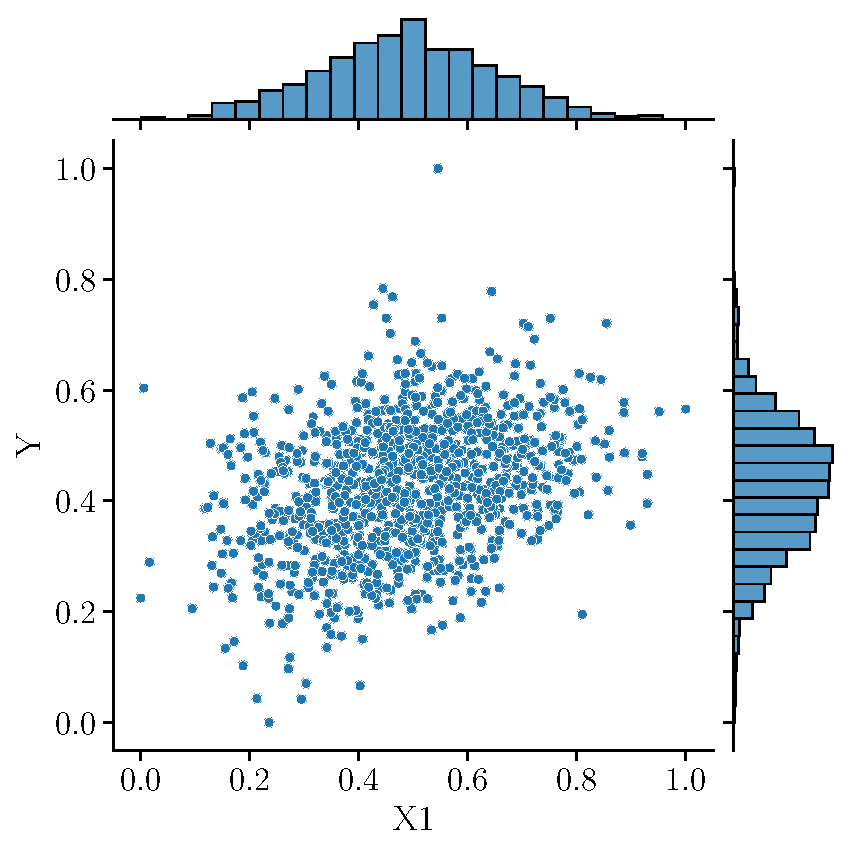
\includegraphics[width=0.32\textwidth]{./part2/figures/SIS/cathare_jointplot_X1.pdf}
%  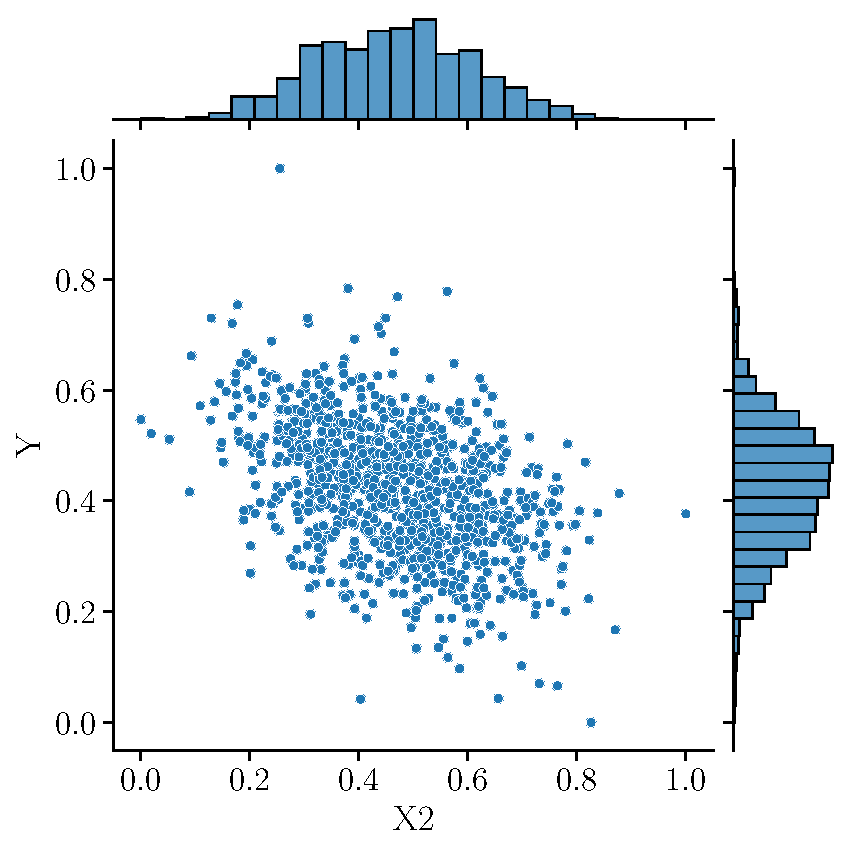
\includegraphics[width=0.32\textwidth]{./part2/figures/SIS/cathare_jointplot_X2.pdf}\\
%  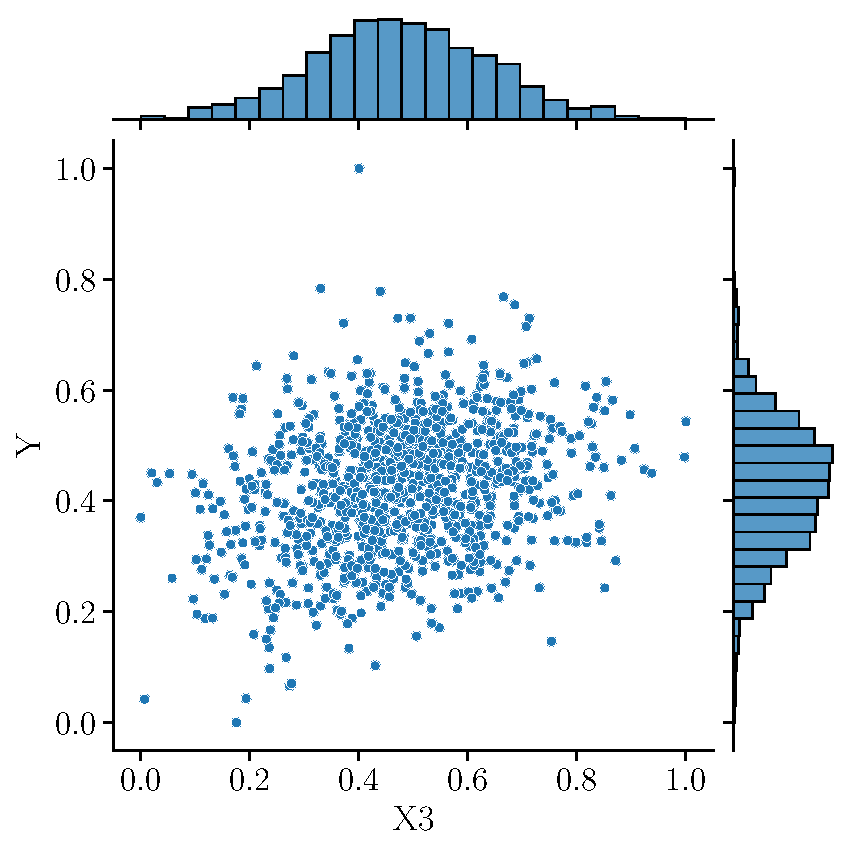
\includegraphics[width=0.32\textwidth]{./part2/figures/SIS/cathare_jointplot_X3.pdf}
%  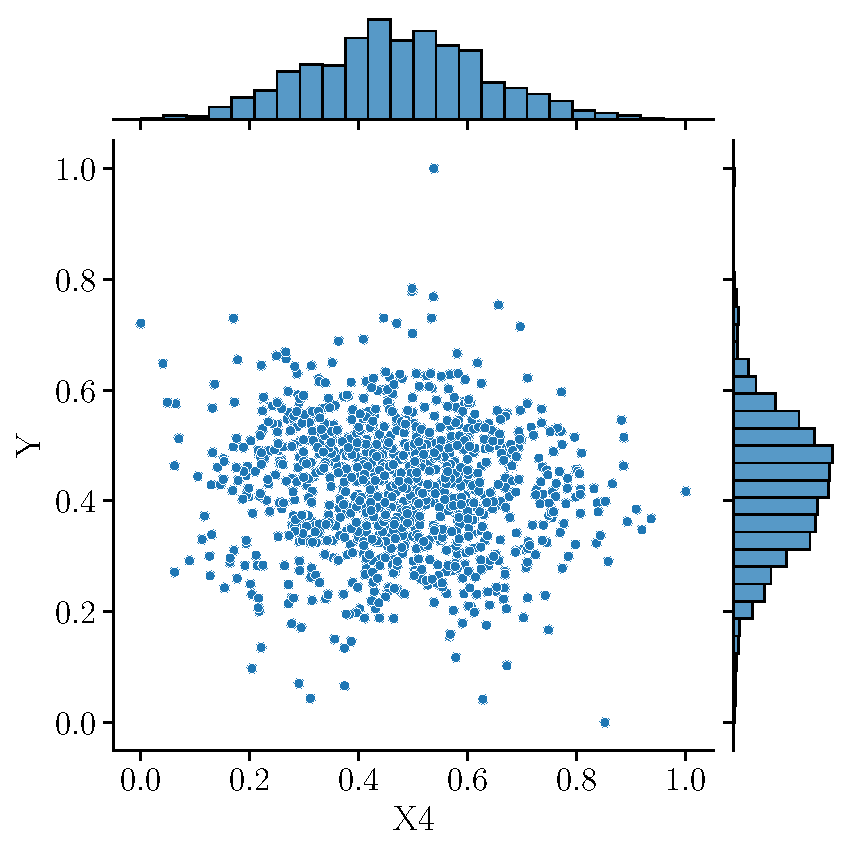
\includegraphics[width=0.32\textwidth]{./part2/figures/SIS/cathare_jointplot_X4.pdf}
%  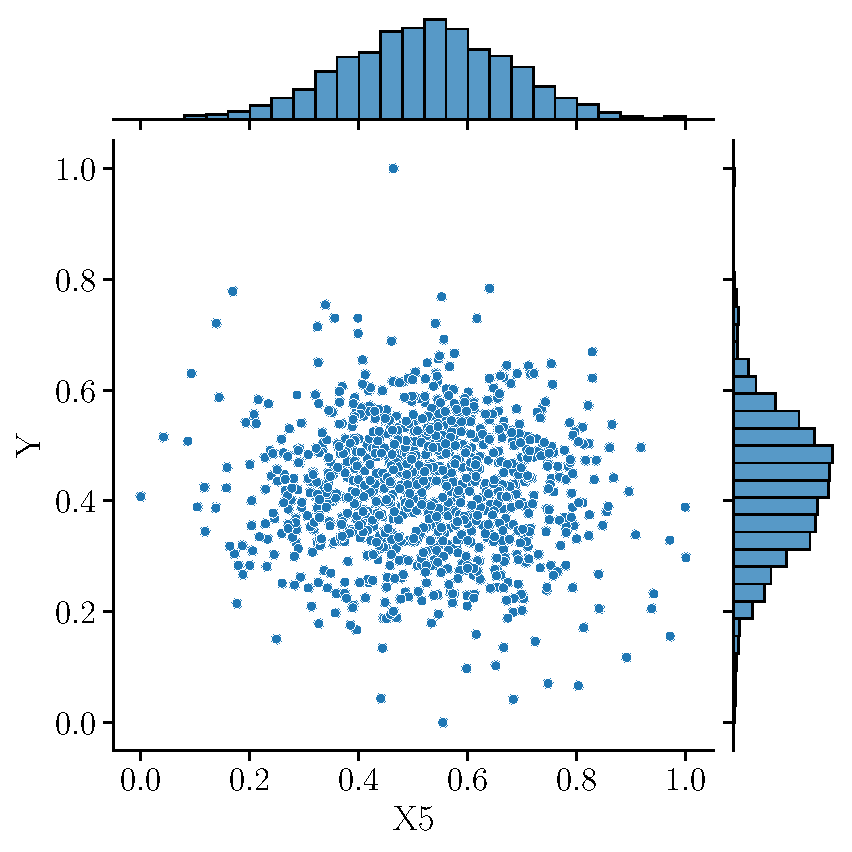
\includegraphics[width=0.32\textwidth]{./part2/figures/SIS/cathare_jointplot_X5.pdf}\\
%  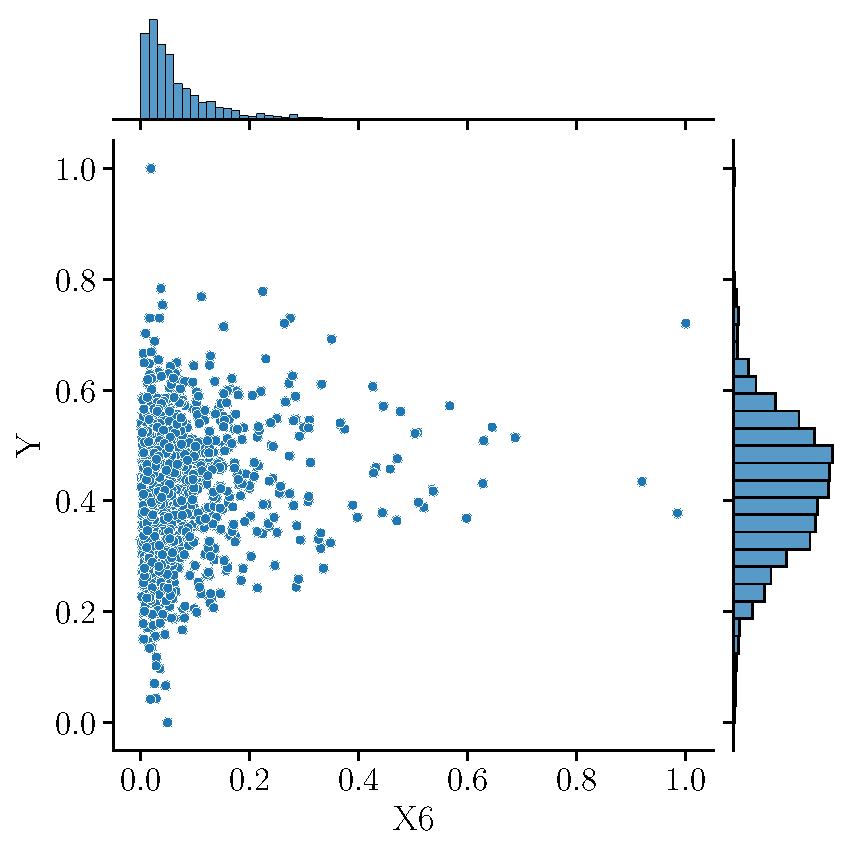
\includegraphics[width=0.32\textwidth]{./part2/figures/SIS/cathare_jointplot_X6.pdf}
%  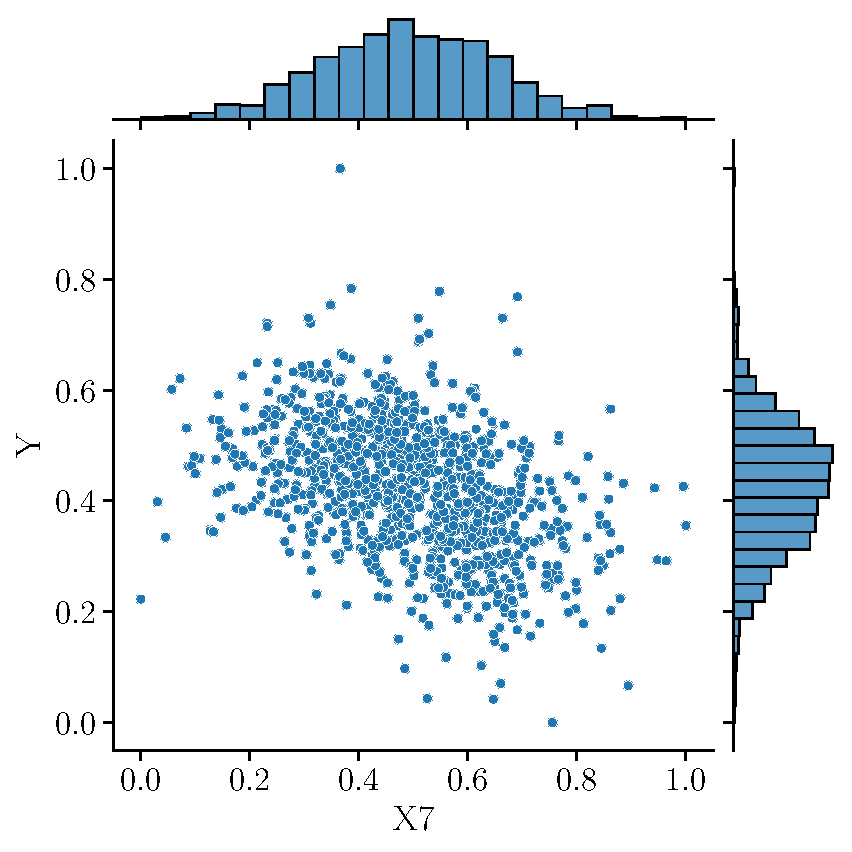
\includegraphics[width=0.32\textwidth]{./part2/figures/SIS/cathare_jointplot_X7.pdf}
%  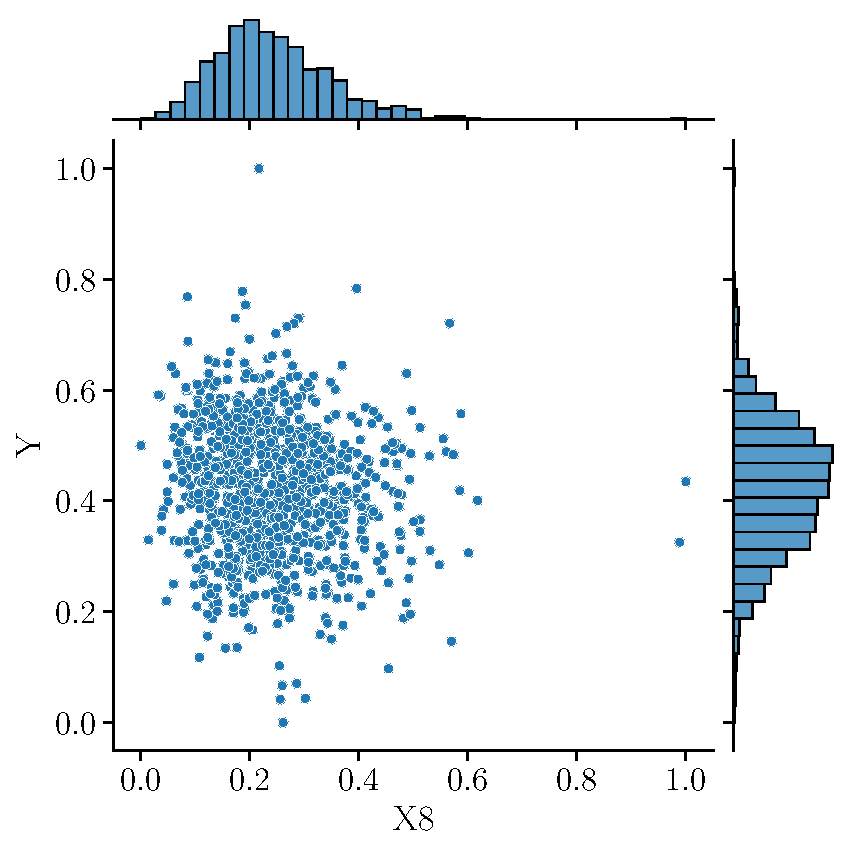
\includegraphics[width=0.32\textwidth]{./part2/figures/SIS/cathare_jointplot_X8.pdf}\\
%  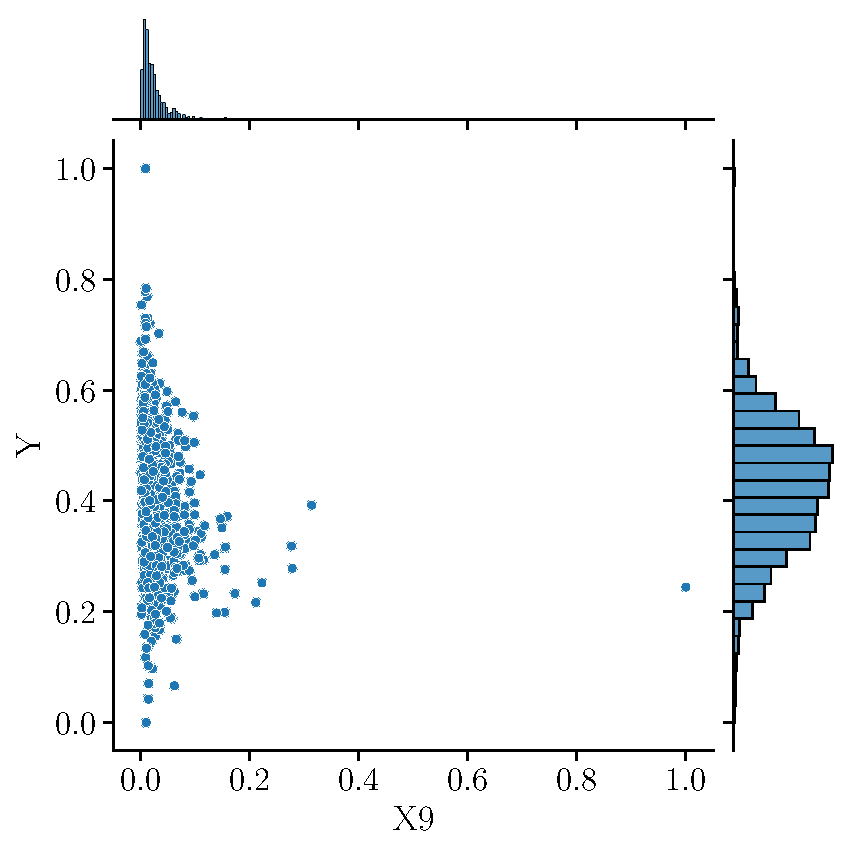
\includegraphics[width=0.32\textwidth]{./part2/figures/SIS/cathare_jointplot_X9.pdf}
%  \caption{test case CATHARE: inputs output scatter plots ($N=10^3$) }
%  \label{fig:cathare_paiplot}
%\end{figure}
In the following, an existing Monte Carlo sample $\bZ_N$ of $N=1\,000$ points in $\R^{53}$ is used, that corresponds to $53$ independent random input configurations (see \citealp{ioobou10} for details). 
The output of the CATHARE2 code at these $N$ points is also available. 
To reduce the dimensionality of this dataset, a sensitivity analysis \citep{daveiga_iooss_2021} screens the inputs that do not impact the output significantly. 
This dimension-reduction step relies on the Hilbert-Schmidt Independence Criterion (HSIC), which is known as a powerful tool to perform input screening from a single sample of inputs and output values without reference to any specific ML regression model \citep{daveiga_2015}. 
HSIC-based statistical tests and their associated $p$-values are used to identify (with a $5\%$-threshold) inputs on which the output is significantly dependent (and therefore, also those of little influence). 
They were successfully applied to similar datasets from thermal-hydraulic applications in \citet{marrel_chabridon_2021,marrel_iscream_2022}. 
The screened dataset only includes $10$ influential inputs, over which the candidate set $\bX_N$ used for the construction of the test-set $\bX_n$ (and therefore of the complementary training set $\bX_{N-n}$) is defined. 
%An input-output scatter plot is presented in \fig{fig:cathare_paiplot}, showing that indeed the retained factors are correlated with the code output. 
The marginal distributions are shown as histograms along the axes of the plots.

To include RCV in the methods to be compared, many (here, $R=1\,000$) different models $\eta_m$ must be constructed for each considered design size $m$. 
Since Gaussian Process regression proved to be too expensive for this purpose, the comparatively cheaper Partial Least Squares (\abv{pls}) method \citep{wolsjo01} is used. 
For each given training set, the model obtained is a sum of monomials in the 10 input variables. 
Note that models constructed with different training sets may involve different monomials and have different numbers of monomial terms. 


%============================================================%
\subsection{Benchmark results and analysis}
%============================================================%

\fig{fig:cathareC2_benchmark} compares various ways of extracting an $n$-point test set from an $N$-point dataset to estimate model predictivity, for different splitting ratios $n/N\in\{0.1,0.15,0.2,\ldots,0.9\}$. 

Consider RCV first. For each value of $r_n=n/N$, the empirical distribution of $Q^2_{RCV}$ obtained from $R=10^3$ random splittings of $\bX_N$ into $\bX_m\cup\bX_n$ is summarized by a boxplot. 
Depending on $r_n$, three behaviors are roughly distinguished. 
For $0.1 \leq r_n \lesssim 0.3$ the distribution is bi-modal, with the lower mode corresponding to unlucky test-set selections leading to poor performance evaluations. 
When $0.3 \lesssim n/N \lesssim 0.7$, the distribution looks uni-modal, revealing a more stable performance evaluation. 
Note that this is (partly) in line with the recommendations discussed in Section~\ref{sec:c5_intro}. 
For $r_n \gtrsim 0.7$, the variance of the distribution increases with $r_n$: many unlucky training sets lead to poor models. 
Note that the median of the empirical distribution slowly decreases as $r_n$ increases, which is consistent with the intuition that the model predictivity should decrease when the size of the training set decreases. 

For completeness, the red diamond represented on the left of \fig{fig:cathareC2_benchmark} the value of $Q^2_{\mathrm{LOO}}$ computed by LOO cross-validation. 
In principle, being computed using the entire dataset, this value should establish an upper bound on the quality of models computed with smaller training sets. 
This is indeed the case for small training sets (rightmost values in the figure), for which the predictivity estimated by LOO is above the majority of the predictivity indexes calculated. 
But at the same time, LOO cross-validation tends to overestimate the errors, which explains the higher predictivity estimated by some other methods when $m=N-n$ is large enough.

Compare now the behavior of the two MMD-based algorithms of Section \ref{sec:val_sampling}, $\widehat Q^2_n$ (un-weighted) and $Q_{n*}^2$ (weighted) are plotted using solid and dashed lines, respectively, for both kernel herding (in blue) and support points (in orange). 
FSSF test sets are not considered, as the application of an iso-probabilistic transformation imposes knowledge of the input distribution, which is not known for this example. 
Compare first the unweighted versions of the two MMD-based estimators. 
For small values of the ratio $r_n$, $0.1 \lesssim r_n \lesssim 0.45$, the relative behavior of support points and kernel herding coincides with what was observed in the previous section, 
support points (solid orange line) estimating a better performance than kernel herding (solid blue line), which, moreover, is close to the median of the empirical distribution of $Q^2_{RCV}$. 
However, for $r_n \geq 0.5$, the dominance is reversed, support points estimating a worse performance than kernel herding. 

As $r_n$ increases up to $r_n \lesssim 0.7$ the solid orange and blue curves crossover, and it is now $\widehat Q^2_n$ for kernel herding that approximates the RCV empirical median, while the value obtained with support points underestimates the predictivity index. 
Also, note that for (irrealistic) very large values of $r_n$ both support points and kernel herding estimate lower $Q^2$ values, which are smaller than the median of the RCV estimates.

Let us now focus on the effect of residual weighting, i.e., in estimators $Q_{n*}^2$ which use the weights computed by the method of Subsection~\ref{sec:weighting}, shown in dashed lines in Figure \ref{fig:cathareC2_benchmark}. 
First, note that while kernel herding weighting leads, as in the previous section, to higher estimates of the predictivity (compare solid and dashed blue lines), this is not the case for support points (solid and dashed orange curves), which, for small split ratios, produces smaller estimates when weighting is introduced. 
In the large $r_n$ region, the behavior is consistent with what was previously presented, weighting inducing an increase of the estimated predictivity. 
It is remarkable -- and rather surprising -- that $Q_{n*}^2$ for support points (the dashed orange line) does not present the discontinuity of the uncorrected curve. 

The sum $\sum_{i=1}^n w_i^*$ of the optimal weights of support points and kernel herding \eq{Eq:weights} is shown in \fig{fig:catharec2_weights} (orange and blue curves, respectively). 
The slow increase with $n/N$ of the sum of kernel-herding weights (blue line) is consistent with the increase of the volume of the input region around each validation point when the size of the training set decreases. 
The behavior of the sum of weights is more difficult to interpret for support points (orange line) but is consistent with the behavior of $Q_{n*}^2$ on \fig{fig:cathareC2_benchmark}. 
Note that the energy-distance kernel \eq{eq:kE} used for support points cannot be used for the weighting method of Subsection~\ref{sec:weighting} as $K_E$ is not positive definite but only conditionally positive definite. 
A full understanding of the observed curves would require a deeper analysis of the geometric characteristics of the designs generated by the two MMD methods, in particular of their interleaving with the training designs, which is not compatible with the space constraints of this manuscript. 

While a number of unanswered points remain, in particular how deeply the behaviors observed may be affected by the poor predictivity resulting from the chosen PLS modeling methodology, the example presented in this section shows that the construction of test sets via MMD minimization and estimation of the predictivity index using the weighted estimator $Q_{n*}^2$ is promising as an efficient alternative to RCV: at a much lower computational cost, it builds performance estimates based on independent data the model developers may not have access to. 
Moreover, kernel herding proved, in the examples studied in this manuscript, to be a more reliable option for designing the test set, exhibiting a behavior that is consistent with what is expected, and very good estimation quality when the residuals over the design points are appropriately weighted.

\begin{figure}
  \centering
  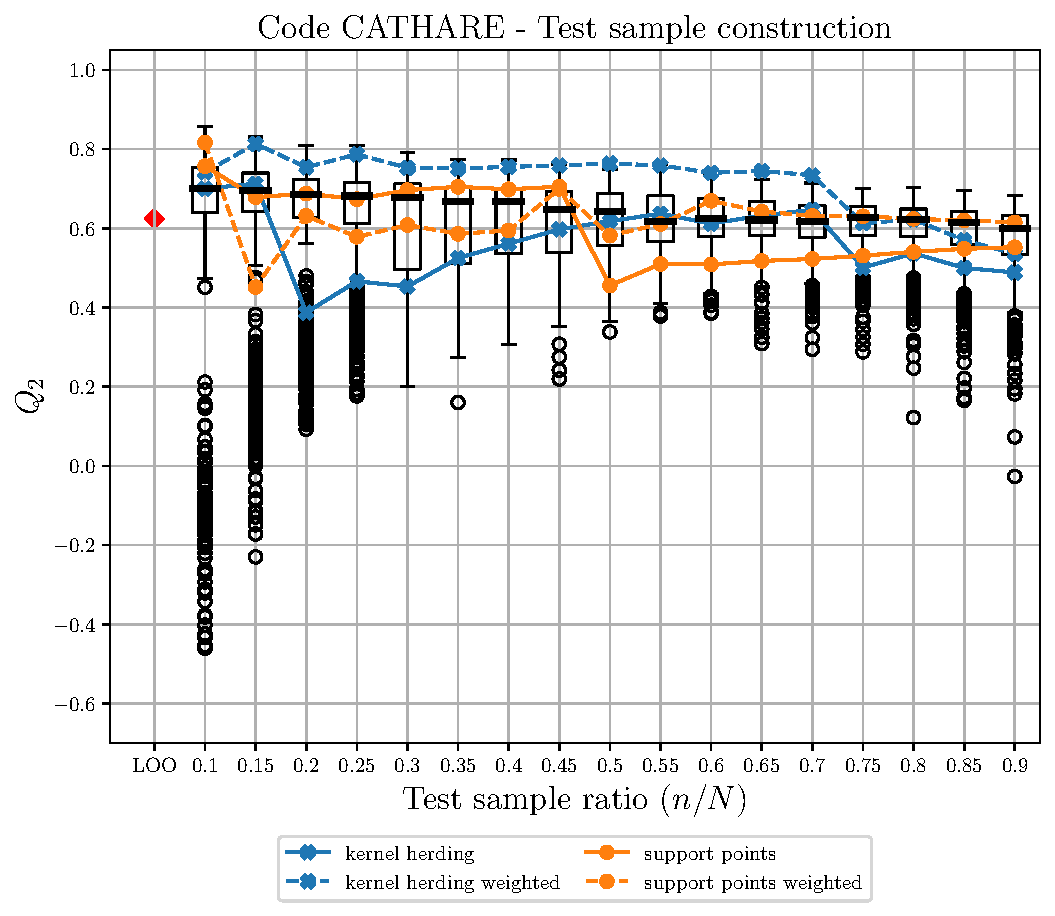
\includegraphics[width=0.7\textwidth]{./part2/figures/SIS/cathareC2.pdf}
  \caption{test case CATHARE: estimated $Q^2$. The box plots are for random cross-validation, and the red diamond (left) is for $Q^2_{\mathrm{LOO}}$.}
  \label{fig:cathareC2_benchmark}
\end{figure}

\begin{figure}
  \centering
  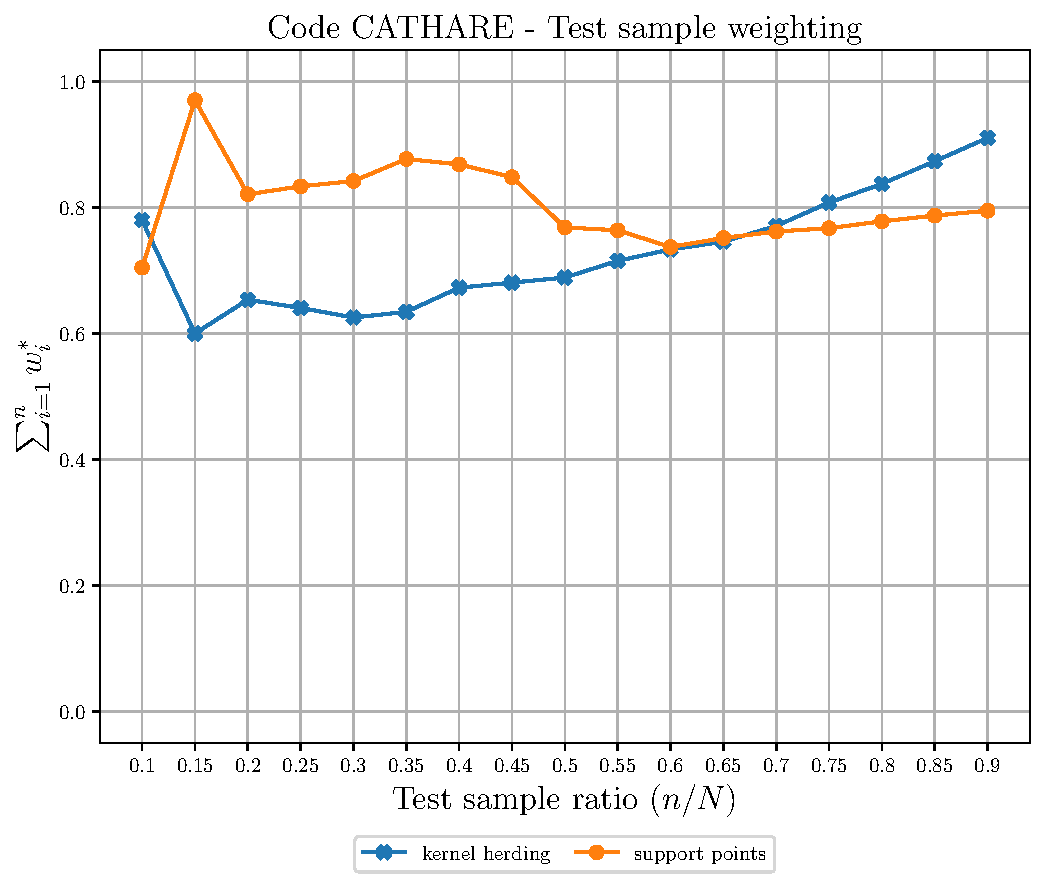
\includegraphics[width=0.6\textwidth]{./part2/figures/SIS/cathareC2_weights.pdf}
  \caption{test case CATHARE: sum of the weights \eq{Eq:weights}.}
  \label{fig:catharec2_weights}
\end{figure}




%============================================================%
%============================================================%
\section{Conclusion}\label{sec:val_conclusion}
%============================================================%
%============================================================%

Our study shows that ideas and tools from the design of experiment framework can be transposed to the problem of test-set selection. 
This chapter explored approaches based on support points, kernel herding and FSSF, considering the incremental construction of a test set (\textit{i}) either as a particular space-filling design problem, where design points should populate the holes left in the design space by the training set, or (\textit{i}) from the point of view of partitioning a given dataset into a training set and a test set. 

A numerical benchmark has been performed for a panel of test cases of different dimensions and complexity. 
Additionally to the usual predictivity coefficient, a new weighted metric (see \citealp{pronzato_rendas_2021}) has been proposed and shown to improve the assessment of the predictivity of a given model for a given test set. 

This weighting procedure appears very efficient for interpolators, like Gaussian process regression models, as it corrects the bias when the points in the test set used to predict the errors are far from the training points. 
For the first three test cases (Section~\ref{sec:val_res1}), pairing one iterative design method with the weight-corrected estimator of the predictivity coefficient $Q^2$ shows promising results as the estimated $Q^2$ characteristic is close to the true one even for test-sets of moderate size. 

Weighting can also be applied to models that do not interpolate the training data. 
For the industrial test case of Section~\ref{sec:val_res2}, the true $Q^2$ value is unknown, but the weight-corrected estimation $Q_{n*}^2$ of $Q^2$ is close to the value estimated by Leave-One-Out cross-validation and to the median of the empirical distribution of $Q^2$ values obtained by random $k$-fold cross-validation. 
At the same time, estimation by $Q_{n*}^2$ involves a much smaller computational cost than cross-validation methods and uses a dataset fully independent of the one used to construct the model. 

To each of the design methods considered to select a test set a downside can be attached. 
FSSF requires knowledge of the input distribution to be able to apply an iso-probabilistic transformation if necessary; it tends to select many points along the boundary of the candidate set considered. 
Support points require the computation of the $N(N-1)/2$ distances between all pairs of candidate points, which implies significant memory requirements for large $N$; the energy-distance kernel on which the method relies cannot be used for the weighting procedure. 
Finally, the efficient implementation of kernel herding relies on analytical expressions for the potentials $P_{\pi}$, see Appendices A and B, which are available for particular distributions (like the uniform and the normal) and kernels (like Matérn) only. 
The great freedom in the choice of the kernel $K$ gives a lot of flexibility, but at the same time implies that some non-trivial decisions have to be made; also, the internal parameters of $K$, such as its correlation lengths, must be specified. 
Future work should go beyond empirical rules of thumb and study the influence of these choices.

Numerical tests were only computed with independent inputs. 
Kernel herding and support points are both well suited for probability measures not being equal to the product of their marginals, which is a frequent case in real datasets. 
Note only incremental constructions were considered, as they allow to stop the validation procedure as soon as the estimation of the model predictivity is deemed sufficiently accurate, but it is also possible to select several points at once, using support points \citep{mak_joseph_2018}, or MMD minimization in general \citep{teymur_gorham_2021}. 

Further developments around this work could be as follows. 
Firstly, the incremental construction of a test set could be coupled with the definition of an appropriate stopping rule, in order to decide when it is necessary to continue improving the model (possibly by supplementing the initial design with the test set, which seems well suited to this). 
The $\MMD_{\Kbarbar}(\zeta_n^*,\pi)$ of Subsection~\ref{sec:weighting} could play an important role in the derivation of such a rule. 
Secondly, the approach presented gives equal importance to all the $d$ inputs. 
However, it seems that inputs with a negligible influence on the output should receive less attention when selecting a test set. 
A preliminary screening step that identifies the significant inputs would allow the test-set selection algorithm to be applied to these variables only. 
For example, when a $\bX_N\subset\R^d$ dataset is to be partitioned into $\bX_m\cup\bX_n$, one could use only $d'<d$ components to define the partition, but still use all $d$ components to build the model and estimate its (weighted) $Q^2$. 
Note, however, that this would imply a slight violation of the conditions mentioned in the introduction, as it renders the test set dependent on the function observations. 

Finally, in some cases, the probability measure $\pi$ is known up to a normalizing constant. 
The use of a Stein kernel then makes the potential $P_{K,\pi}$ identically zero \citep{chen_2018_stein_points}, which would facilitate the application of kernel herding. 
Also, more complex problems involve functional inputs, like temporal signals, images, or categorical variables; the application of the methods presented to kernels specifically designed for such situations raises challenging issues. 






